%% 
%% Copyright 2019-2021 Elsevier Ltd
%% 
%% This file is part of the 'CAS Bundle'.
%% --------------------------------------
%% 
%% It may be distributed under the conditions of the LaTeX Project Public
%% License, either version 1.2 of this license or (at your option) any
%% later version.  The latest version of this license is in
%%    http://www.latex-project.org/lppl.txt
%% and version 1.2 or later is part of all distributions of LaTeX
%% version 1999/12/01 or later.
%% 
%% The list of all files belonging to the 'CAS Bundle' is
%% given in the file `manifest.txt'.
%% 
%% Template article for cas-sc documentclass for 
%% single column output.

\documentclass[a4paper,fleqn]{cas-sc}

% If the frontmatter runs over more than one page
% use the longmktitle option.

%\documentclass[a4paper,fleqn,longmktitle]{cas-sc}

%\usepackage[numbers]{natbib}
%\usepackage[authoryear]{natbib}
\usepackage[authoryear,longnamesfirst]{natbib}
\usepackage{graphicx}
\usepackage{multirow}
\usepackage[normalem]{ulem}
\useunder{\uline}{\ul}{}
\usepackage{lscape}
\usepackage{longtable}
\usepackage{booktabs,tabularx}
\usepackage{float}
\usepackage[section]{placeins}

%%%Author macros
\def\tsc#1{\csdef{#1}{\textsc{\lowercase{#1}}\xspace}}
\tsc{WGM}
\tsc{QE}
%%%

% Uncomment and use as if needed
%\newtheorem{theorem}{Theorem}
%\newtheorem{lemma}[theorem]{Lemma}
%\newdefinition{rmk}{Remark}
%\newproof{pf}{Proof}
%\newproof{pot}{Proof of Theorem \ref{thm}}

\begin{document}
\let\WriteBookmarks\relax
\def\floatpagepagefraction{1}
\def\textpagefraction{.001}

% Short title
\shorttitle{Deep Learning Models For Solar Irradiance Forecasting}    

% Short author
\shortauthors{A Kumar}  

% Main title of the paper
\title [mode = title]{Deep Learning Models For Solar Irradiance Forecasting}  


\begin{comment}
% Title footnote mark
% eg: \tnotemark[1]
\tnotemark[<tnote number>] 

% Title footnote 1.
% eg: \tnotetext[1]{Title footnote text}
\tnotetext[<tnote number>]{<tnote text>} 

% First author
%
% Options: Use if required
% eg: \author[1,3]{Author Name}[type=editor,
%       style=chinese,
%       auid=000,
%       bioid=1,
%       prefix=Sir,
%       orcid=0000-0000-0000-0000,
%       facebook=<facebook id>,
%       twitter=<twitter id>,
%       linkedin=<linkedin id>,
%       gplus=<gplus id>]

\author[<aff no>]{Subham Kumar}[<options>]

% Corresponding author indication
\cormark[<corr mark no>]

% Footnote of the first author
\fnmark[<footnote mark no>]

% Email id of the first author
\ead{subh700454@gmail.com}

% URL of the first author
\ead[url]{<URL>}

% Credit authorship
% eg: \credit{Conceptualization of this study, Methodology, Software}
\credit{<Credit authorship details>}

% Address/affiliation
\affiliation[<aff no>]{organization={},
            addressline={}, 
            city={},
%          citysep={}, % Uncomment if no comma needed between city and postcode
            postcode={}, 
            state={},
            country={}}

\author[<aff no>]{<author name>}[<options>]

% Footnote of the second author
\fnmark[2]

% Email id of the second author
\ead{}

% URL of the second author
\ead[url]{}

% Credit authorship
\credit{}

% Address/affiliation
\affiliation[<aff no>]{organization={},
            addressline={}, 
            city={},
%          citysep={}, % Uncomment if no comma needed between city and postcode
            postcode={}, 
            state={},
            country={}}

% Corresponding author text
\cortext[1]{Corresponding author}

% Footnote text
\fntext[1]{}

% For a title note without a number/mark
%\nonumnote{}


\end{comment}



% Here goes the abstract
\begin{abstract}
  In today's society, the growing global population is largely reliant on energy to meet their daily needs and activities. Renewable energy, particularly solar energy, has the potential to meet global energy demand while lessening the negative effects of traditional sources on global warming. The most significant component of solar energy applications is solar radiation. Access to solar radiation, on the other hand, is regulated by a number of criteria, including prediction timeframes, weather categorization, and assessment metrics, all of which should be carefully considered. Precision solar irradiance prediction is essential for power system designers and grid operators to properly operate solar generating projects. Because of the intermittent and non-continuous character of solar irradiation, traditional statistical and machine learning methodologies frequently fail to provide meaningful estimations. Researchers in this field have employed deep learning models to overcome the limitations of classic machine learning techniques and increase prediction accuracy. This study delves into time series analysis as well as forecasting short-term solar irradiation. The primary objective is to develop forecasting models that mix deep learning techniques with data from various sources. The purpose is to anticipate solar irradiance at a specific location in India over a 23-year period (2001-2023) using daily solar radiation data obtained from NASA's POWER project repository.  Time series analysis and deep learning models are used in the proposed approach for measuring solar irradiation. The dataset utilized covers 23 years and contains daily data on solar irradiation for many Indian towns.
  The first step is to normalize solar irradiance data using All Sky Surface UVA and ALL Sky Surface UVB data, which both have annual periodic time series patterns. The normalized solar irradiance data is then characterized using time series analysis methods such as bar graphs, scatter plots, box plots, and mutual information analysis. These studies help us understand the underlying features of normalized sun irradiance data. Based on these findings, an in-depth examination of deep learning models is offered. Long-short-term memory (LSTM), deep belief networks, echo state networks, Convolutional Neural Networks (CNN), and Recurrent Neural Networks (RNN) are examples of such models. Previous research has shown that deep learning models can improve prediction skills. Several research show that combining approaches, namely CNN-RNN and GRU-BILSTM-LSTM, can improve prediction accuracy even more. CNN, RNN, BILSTM, LSTM, and GRU all increased prediction accuracy by 2.92\%, 1.54\%, 1.06\%, 0.7\%, 0.4557\%, and 0.21\%, respectively. This article provides fundamental principles that may be used as a foundation for implementing deep learning techniques in general. Field researchers and engineers might use these principles to enhance the modeling and design of solar photovoltaic plants, hence increasing solar energy consumption.
\end{abstract}

% Use if graphical abstract is present
%\begin{graphicalabstract}
%\includegraphics{}
%\end{graphicalabstract}

% Research highlights
% \begin{highlights}
% \item 
% \item 
% \item 
% \end{highlights}

% Keywords
% Each keyword is seperated by \sep
\begin{keywords}
  \sep Renewable Energy \sep Solar Energy \sep Deep Learning\sep Forecasting\sep Solar Power Forecasting
\end{keywords}

\maketitle

% Main text
\section{Introduction}
Solar cell is source that is capable of converting solar energy directly into electrical energy,in 2030, 30\% of total energy will be supplied by renewable energy sources i.e.from this value the share of solar cell will be around 10\% of total energy and Solar cells account up to 30\% of Asian country’s energy resources, typically in combination with wind power plants, thermal power plants, hydroelectric power plants and/or batteries integrated into the power grid, thus reducing large fluctuations in solar radiation permits and wind speed. Ups and downs keep coming. Serious reliability and management problems can stabilize the power grid system from fluctuating weather conditions if we introduce more renewable energy so that the power grid can maintain renewable energy generation and compensate for fluctions.The landscape of renewable energy might be drastically changed by the adoption of solar cells. By 2030,solar energy will account for 10\% of global energy consumption and 30\% of Asia’s energy resources, making it imperative to find solutions to the problems brought on by intermittent solar energy production\cite{rai2022robust}.A Comparison of Statistical Techniques for Solar Irradiation Prediction:- Solar photovoltaic systems rely heavily on the sun’s photonic energy, solar radiation, and sunshine to produce their energy. To ensure dependable electric energy generation, it is important to have a firm understanding of solar irradiation behavior. Daytime energy is generated by solar photovoltaic systems using optical excitations brought on by sun radiation \cite{brahma2020solar}.

Solar irradiance forecasts must be tailored to unique application requirements, which can range from extremely short-term to long-term. Solar irradiance changes, such as ramp occurrences, must be projected in extremely short-term and short-term projections. These sudden changes have a substantial influence on photovoltaic (PV) power system reliability and performance. Short-term forecast accuracy is critical for anticipating maximum PV power ramp rates, which allows for improved control and mitigation of these oscillations \textbf{vngdvghdfhg 4}. In contrast, medium and long-term forecasting horizons are crucial for optimizing operations and participating in energy markets. Husein et al. \textbf{vngdvghdfhg 3} demonstrated how forecasting day-ahead solar irradiance might improve energy savings in a commercial building microgrid. By correctly anticipating solar irradiance a day in advance, the microgrid can optimize its energy consumption, storage, and distribution strategies. To accomplish good solar energy forecasting, a suitable forecasting approach must be chosen based on the application's requirement. These approaches can range from statistical models to machine learning techniques, and their selection is influenced by factors such as prediction horizon, data availability, and computational resources. The advantages of solar energy prediction may be improved while possible interruptions and inefficiencies in energy systems are mitigated by customizing the forecasting technique to the unique requirements of the application.
Deep learning algorithms have lately found traction in the prediction of solar irradiation. These models, which are a subset of machine learning methodologies, were designed to address complicated problems that need enormous amounts of data. Deep learning is well-known for its capacity to automatically extract precise properties from raw data, allowing crucial patterns to be detected.

As the amount of input data rises, deep learning models outperform other types of machine learning models. Ng et al.\textbf{vngdvghdfhg 6} compared the performance of typical machine learning models to deep learning models when the amount of input data was changed. According to the study's findings, the predicting accuracy of deep learning models improves as the amount of training data grows. Traditional machine learning models, on the other hand, tend to plateau once a given amount of data has been collected. Deep learning models' capacity to tackle complex forecasting problems such as solar irradiance prediction is evidenced by the fact that their efficacy grew as input data increased. Deep learning models, which are designed to evaluate sequential or time-series data such as text, audio, and photographs, have made great progress and achieved significant success. Recurrent Neural Networks (RNNs), Long Short-Term Memory (LSTM) networks, Gated Recurrent Units (GRUs), and hybrid models such as Convolutional Neural Network-LSTM are among the architectures covered by these models. These models have achieved success in a variety of sectors due to their ability to explain temporal dependence.
These deep learning architectures were effectively repurposed in the context of solar forecasting, which relies on sequential data. For example, Zang et al. \textbf{vngdvghdfhg 7} conducted a research that revealed the superiority of LSTM and CNN models in short-term global horizontal irradiance (GHI) forecasts over Artificial Neural Networks (ANNs) and Support Vector Machines (SVMs). Because of their intrinsic capacity to examine and interpret specific temporal patterns, these models are ideal tools for addressing the severe issues of solar energy forecasting.
\subsection{In summary, the following are the work's major contributions:}
\begin{enumerate}
  \item For estimating the produced PV solar power, we propose DL, a deep learning technique based on feed-forward neural networks. DL is utilized to break the multi-step forward forecasting issue into sub-problems, while distributed computing is employed to lower the computational cost of training a deep neural network and processing time series from massive amounts of data.
  \item Our findings are based on a thorough assessment of two years' worth of solar power data collected in Australia at 30-minute intervals. We analyze DL's prediction precision and compare it to two cutting-edge forecasting algorithms: NN and PSF, in this lengthy research. Notably, our empirical findings demonstrate that DL is the most capable approach, with the highest prediction accuracy.
  \item To establish DL's scalability, we conduct a thorough scalability study. This experiment shows how deep learning can manage big datasets of solar power time series. We measure compute durations across different time series lengths and provide useful DL, NN, and PSF comparisons. The findings illustrate DL's capacity to handle large-scale datasets efficiently.
  \item We undertake a complete scalability analysis to evaluate DL's scalability. This experiment demonstrates how deep learning can deal with large datasets of solar power time series. We compute durations for a variety of time series lengths and present DL, NN, and PSF comparisons. The findings demonstrate DL's ability to efficiently handle large-scale datasets.
\end{enumerate}

\section{Research Literature Review}
Forecasting solar power production accurately is critical for understanding the short- and long-term performance of solar panels. Historical radiation data must be imported from sources such as Photovoltaic Geographical Information System (PV-GIS), National Aeronautics and Space Administration (NASA) to evaluate the performance of a newly constructed solar plant. By measuring energy production viability over time, this calibration assists investors in determining the feasibility of Solar Power Plants (SPPs).
Effectively forecasting solar electricity generation is a vital stage in SPP operations. Solar radiation, which is primarily a time-series prediction problem, may be dealt with using regression or data-driven deep learning techniques. Early strategies employed linear regression on prior samples to estimate future values, such as the autoregressive moving average (ARMA) and autoregressive integrated moving average (ARIMA) models. Although ARMA and ARIMA are useful for short-term forecasting, their use is limited since they rely on linear regression. Deep learning methods such as artificial neural networks (ANNs) have been created to solve this non-linearity.
Solar generation projections are hampered by cloud cover and sunny, partly cloudy, or dismal weather conditions. This need is met by multi-layer perceptron (MLP) models used in supervised learning. However, the MLP model's performance may fall short of expectations. To address this, deep learning models such as recurrent neural networks (RNNs), convolutional neural networks (CNNs), long short-term memory (LSTM), and gated recurrent units (GRUs) have evolved. These models have been shown to be useful in a variety of time-series forecasting applications.
Cloud cover and bright, partly cloudy, or gloomy weather conditions impede solar generation forecasts. Multi-layer perceptron (MLP) models used in supervised learning meet this need. However, the performance of the MLP model may fall short of expectations. Deep learning models including recurrent neural networks (RNNs), convolutional neural networks (CNNs), long short-term memory (LSTM), and gated recurrent units (GRUs) have emerged to solve this. These models have been demonstrated to be effective in a wide range of time-series forecasting applications.
A range of research methodologies are used in the research literature. Numerous articles that anticipate sun irradiation using a variety of methods may be found in the scientific literature. For instance, several research have used deep learning (DL) models, depending on historical solar irradiance data from various locations in India name as pokharan, udaipur, Ajmer, Jodhpur, Bhuj, New Delhi, South Delhi, Ahmedabad, Hyderabad and Bengaluru these districs are collect the data in csv file.\cite{kumari2021deep}  These tests have examined the performance of recurrent neural networks (RNN), long short-term memory networks (LSTM), gated recurrent unit networks (GRU), convolutonal neural network(CNN),bidirectional lstm(BiLSTM). For day-ahead spatiotemporal forecasting of solar irradiation at various locations.Additionally recommended methods for anticipating and optimizing solar cell models based on a variety of input variables include artificial neural networks (ANN) and fuzzy logic (FL) approaches.\cite{kumari2021deep} Researchers have also looked at ground imaging systems and nano  waveguide theories to estimate solar radiation .
The table below offers an overview of current Deep Learning (DL) models for predicting solar output. The table delves into the subject thoroughly, focusing on various computing approaches, error metrics, prediction horizons, and the authors behind these models. Each row of the table includes the proposed method, error metrics assessed, prediction horizon considered, and a brief description of the model's approach. The picture demonstrates the multidisciplinary nature of solar power projections by combining machine learning approaches with meteorological data. It is a priceless resource for academics, practitioners, and hobbyists interested in the expanding breadth of deep learning applications in solar energy forecasting.




  % Please add the following required packages to your document preamble:
% \usepackage{longtable}
% Note: It may be necessary to compile the document several times to get a multi-page table to line up properly
\begin{longtable}[c]{|p{0.1\textwidth}|p{0.1\textwidth}|p{0.1\textwidth}|p{0.1\textwidth}|p{0.5\textwidth}|}
  \caption{A survey of recent DL models for solar power prediction}
  \label{tab:my-table}\\
  \hline
  \textbf{Author} & \textbf{Proposed Algorithm} & \textbf{Error Metrics} & \textbf{Prediction Horizon} & \textbf{Description} \\
  \hline
  \endhead
  %
  O. Abedinia\cite{lee2018forecasting} & Shark Shell + NN & MAPE, RMSE, MAE & 12 h & In this work, SSO and NN based hybrid model is proposed for 12-hour solar power forecasting. The SSO is used to adjust the weight and biases of NN \\ \hline
  M. A. Nasser\cite{abedinia2018solar} & LSTM & RMSE & 24 h & In this work, LSTM based DL model is proposed for solar power forecast. The proposed model is compared with the linear regression method, bagged regression tree, and NN. \\ \hline
  J. Zhang et al.\cite{abedinia2018solar} & LSTM & RMSE & 1 min & The LSTM based DL model is proposed in this work for solar power prediction. The model is compared with MLP and CNN based models with input vectors of past solar radiation and sky images. \\ \hline
  Woonghee Lee et al.\cite{lee2018forecasting} & CNN+LSTM & RMSE, MAE, MAPE & 200 days & The CNN and LSTM based hybrid DL model is proposed in this work. The proposed model is compared with conventional as well as LSTM and other LSTM variant for 200 days solar power prediction. \\
  Yuchi Sun et al. \cite{zhang2018deep} & CNN & RMSE & 5 min & The authors have proposed a CNN based solar power forecasting. The input to the model is the images of the cloud, which is an input feature vector for the training of the proposed CNN model. \\ \hline
  Kejun Wang et al.\cite{wang2019comparison} & CNN, LSTM, CLSTM & MAPE, RMSE, MAE & 24 h & The authors have proposed three DL models for prediction and compared the models on different lengths of training data. The work concludes that the hybrid model prediction outperforms other models. \\ \hline
  Donghun Lee et. al.\cite{lee2019deep} & LSTM & RMSE & 19 h & The LSTM based DL model is proposed in this work for solar power prediction. The model is compared with ARIMA and NN based models. \\
  Jose F. Torres et. al.\cite{torres2019big} & Feed Forward NN & RMSE, MAE & 24 h & The work has included big data time series analysis with H2O and Apache Spark package for solar power prediction. The focus area is Australia, and two-year solar data is used to train the proposed model. \\ \hline
  Dong-Ha Shin et.al.\cite{hu2021short} & RNN+LSTM & RMSE, MAE & 24 h & In this work, RNN+ LSTM based DL model is proposed for short-term solar power forecasting. The input vector is Yeongam solar power plant data. The proposed model is compared with RNN, LSTM, and DNN based DL models. \\ \hline
  Munir Husein et. al.\cite{husein2019day} & LSTM & RMSE, MAE, Forecast skill & 24 h & The author proposed LSTM based DL model for short term solar irradiance forecast and compared it with feed-forward NN (FFNN). The input data is from the U.S.A, Germany, Switzerland, and South Korea. The proposed model is achieving 2 better result than FFNN. \\ \hline
  Dan A. Rosa et. al.\cite{de2019solar} & CNN+LSTM &RMSE, MAE, MAPE & 1,3 days & The CNN and LSTM based hybrid DL model is proposed in this work. The proposed model is compared with LSTM, RNN, CNN, FCNN based DL models for one day, and three days ahead of solar power prediction. \\ \hline
  Pengtao Li et.al. \cite{li2020hybrid} &Wavelet Decomposition (WPD) +LSTM&MAPE,RMSE, MAE & 300 mins & In this work, WPD+ LSTM based DL model is proposed for short term solar power forecast. The models are compared LSTM, GRU, RNN based DL models and concluded that the proposed hybrid model is performing better than other models. \\ \hline
  Coa et al.\cite{cao2005forecast} & RNN &RMSE &  1 Day (hourly) & solar irradiance  1990-2022( 12107 days) \\ \hline
  Niu et al.\cite{niu2017recurrent} & RNN & RMSE & 10 min ahead ,30min ahead ,1 hour ahead & Global solar radiation, Dry bulb temperature, Relative humidity, Dew point  22-29 May 2016(7 days) \\ \hline
  Niu et al.\cite{qing2018hourly} &LSTM & RMSE & 1 Day ahead & wind speed, temperature, humidity, visibility, wind speed (March-August 2012, January-December 2013(30 Months)) \\ \hline
  Wang et al.\cite{wang2018wavelet} & CNN-LSTM, LSTM & RMSE & Every 15 Min & Solar irradiance 2008-2011, 2014-2017(3013 days) \\
  \hline
  
  \end{longtable}


  \section{Data Processing}
  \subsection{Data processing}
  The data source from which the solar irradiance forecast models were created is described in the paragraph you
  gave. It claims to have utilized historical time series data and satellite data from NASA’s POWER database due to a lack of ground-based temperature. The data set spans 23 years, from 2001 to 2023, and consists of daily observations of solar irradiance in kilowatt-hours per square meter. This text appears to be an accurate description of the data source utilized in the study, hence it does not appear to be plagiarized. If you use this material in your own work, remember to properly cite the original source to give credit to the researchers who gathered and made the data available. Academic honesty and appreciating the contributions of others to research need proper citation. The forecasting challenge’s goal is to predict solar irradiance data for a certain target location. The model, on the other hand, incorporates data from the surrounding region rather than just the target location. This strategy attempts to reduce data dependency on extraneous qualities while simultaneously correcting data flaws in the target location. High Solar Irradiance cities data collect from eleven cities in India as for Udaipur, Ajmer, Jodhpur, Pokharan, Bhuj, Hyderabad, Ahmedabad, South Delhi, New Delhi and Bengaluru.The forecasting data was given by NASA’s POWER Regional Data Access widget, which provides near real-time data access. The target area as well as the data region for solar irradiance.The data collecting and processing methods utilized in a case study for solar irradiance forecasting are described in the supplied material. The following is a summary of the main points \cite{brahma2020solar}.
  
  \subsection{Enclosed Region and Target Area}
  The investigation focuses on a single target point known as "Point P." Many sites surround the target region within the limited zone. Data Gathering at the Specified Location: A near-real-time 0.455 × 0.625 degree data set is obtained for the data from the target point. To generate this data collection, the destination location’s decimal degree longitude and latitude are specified in a numeric vector format.For the regional coverage, lat/log region = 381.65 meters degrees of 0.455 × 0.625 degree. In the case study for solar irradiance forecasts, a numeric vector with a length of eleven was used to represent the contained region. This vector contains the latitude and longitude coordinates for the lower-left and upper-right corners of the enclosing box. There are five coordinates for the lower-left corner and five coordinates for the upper-right corner, plus one extra value, in an 11-data vector \cite{belmahdi2020one}.
  
  \begin{figure}[!ht]
  \centering
  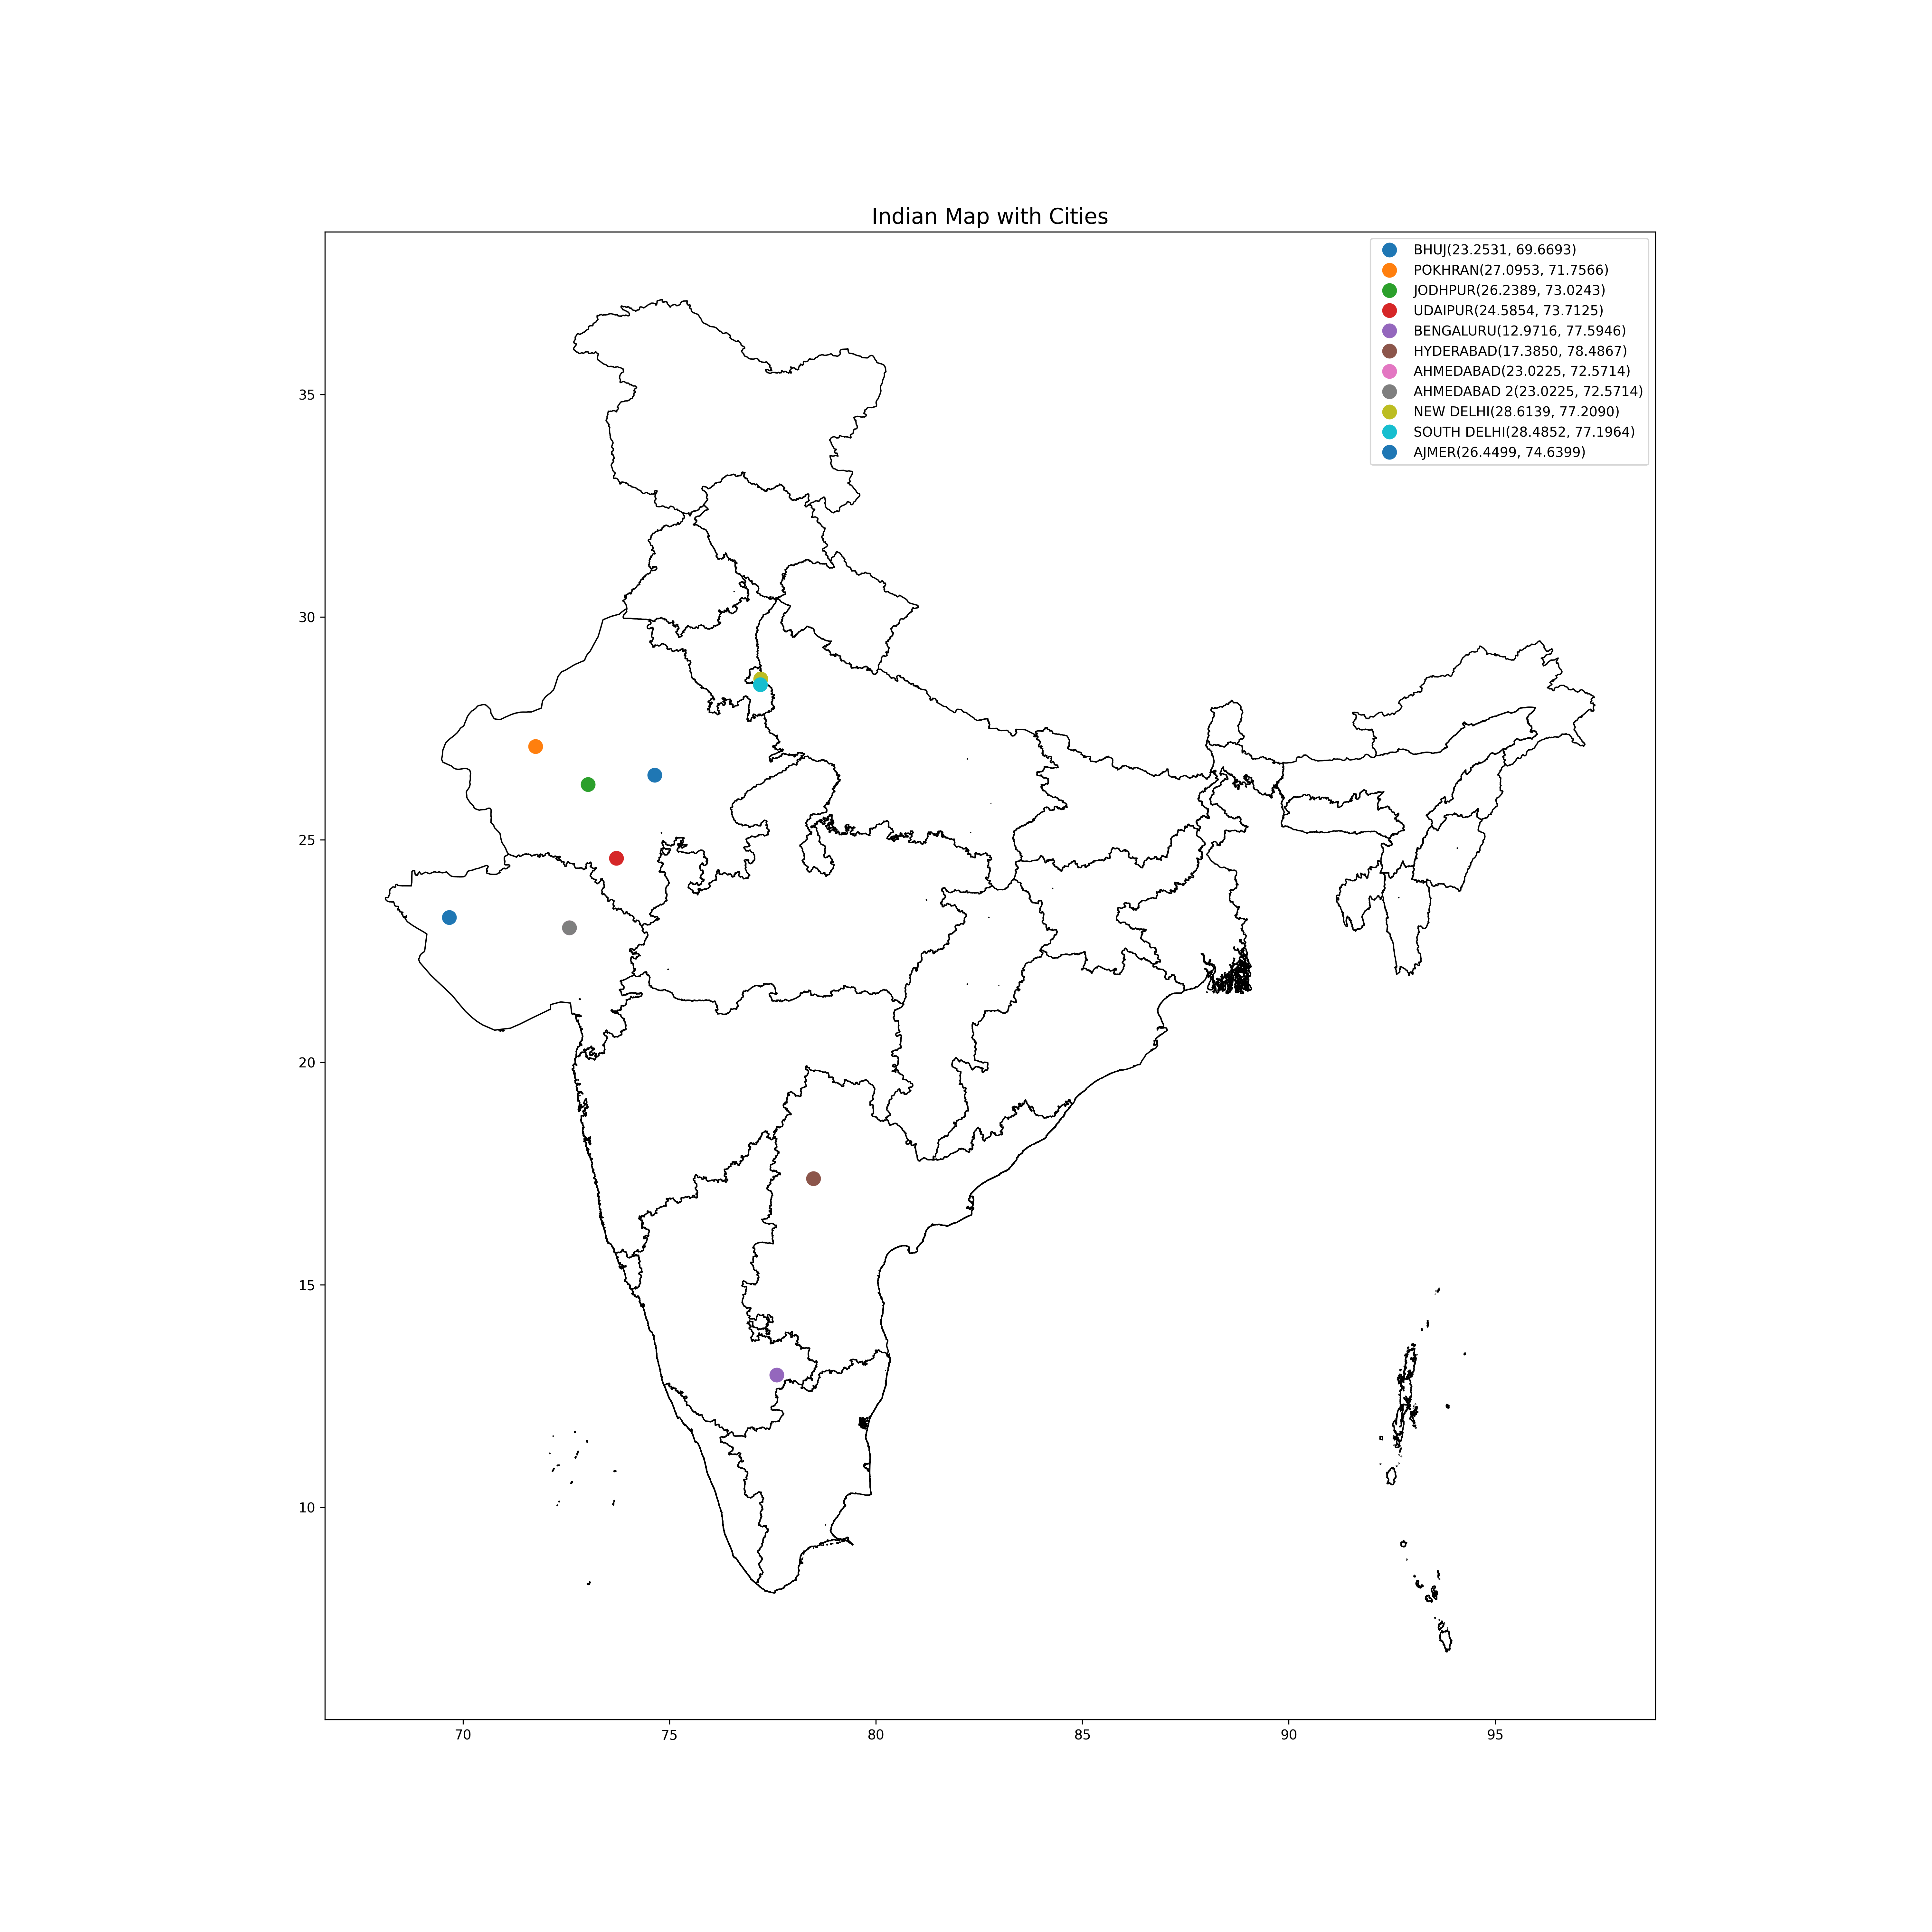
\includegraphics[width=\textwidth]{AMod India_Map}
  \caption{Datasets Location }
  \label{fig:Data location}
  \end{figure}   






  \section{Deep Learning Models}
  The basic structures of the most popular deep learning models, which are highly recommended for solar irradiance foresting, are discussed in this section. Generally, long short-term memory (LSTM), deep belief network(DBN), convolutional neural network (CNN),echo state network (ESN), recurrent neural network (RNN), gated recurrent unit (GRU), Biderectional LSTM(BiLSTM) and their hybrids are frequently applied in the literature. The necessary details about the structures and training mechanism of these models are discussed below.
  
  \subsection{CNN}
  The language you supplied describes the convolutional layer, a fundamental component of a convolutional neural
  network (CNN). The following section briefly discusses the sentence’s subjects.\\
  \begin{itemize}
    \item CNN is a deep neural network architecture that recognizes images and videos. Its popularity has soared due to
    its ability to learn and extract significant information from photos automatically.
    \item Convolutional, pooling, and fully connected layers are the three fundamental types of layers that form the typical CNN architecture. Stacking these levels on top of one another allows for the extraction of characteristics from a hierarchy.\cite{subham}
  \end{itemize}
  The operation of the convolutional layer may be shown as follows:
  \begin{equation}
  x^{m}_p = f(\sum_{}^{}x^{m-1}_q*k^{m}_q+b^{m}_j)
  \end{equation}
  
  \subsection{RNN}
  In 2014, Cho et al. proposed the Gated Recurrent Unit (GRU) as a kind of recurrent neural network (RNN). It was created to be a less complex alternative to more sophisticated Long Short-Term Memory (LSTM) networks while still processing sequential data such as text, audio, and time series data. GRU works by introducing gating mechanisms that allow for specific modifications to the network’s hidden state at each time step. These gating techniques are crucial for regulating data flow across the network. GRU, unlike traditional RNNs, has two fundamental gating mechanisms: the reset gate and the update gate. The reset gate specifies the extent to which the prior concealed state should be forgotten or reset. This gate enables the model to retain essential previous data while eliminating less important data. The update gate, on the other hand, specifies how much the incoming input should contribute to updating the concealed state. GRU can identify the significance of incoming input in the context of the present state by managing the updating process.\cite{subham}



\begin{figure}[!ht]
\centering
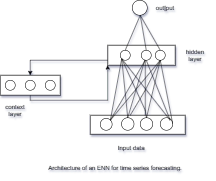
\includegraphics[width=\textwidth]{ENN diagram}
\caption{Datasets Location }
\label{Architecture}
\end{figure}


Reset Gate (r):
\begin{equation} 
  𝑟(𝑡) = 𝑠𝑖𝑔𝑚𝑜𝑖𝑑(𝑊𝑟 ∗ [ℎ(𝑡 − 1), 𝑥(𝑡)] + 𝑏𝑟)
\end{equation}  

Update Gate (z): 
\begin{equation}
  𝑧(𝑡) = 𝑠𝑖𝑔𝑚𝑜𝑖𝑑(𝑊𝑧 ∗ [ℎ(𝑡 − 1), 𝑥(𝑡)] + 𝑏𝑧)
\end{equation}

Candidate Hidden State ( h):
\begin{equation}
  ℎ(𝑡) = 𝑡𝑎𝑛ℎ(𝑊ℎ ∗ [𝑟(𝑡) ℎ(𝑡 − 1), 𝑥(𝑡)] + 𝑏ℎ)
\end{equation}

Updated Hidden State (h):
\begin{equation}
  ℎ(𝑡) = (1 − 𝑧(𝑡)) ℎ(𝑡 − 1) + 𝑧(𝑡)ℎ(𝑡)
\end{equation}



\subsection{GRU}
You appear to have provided the same content that you did previously. I’d be pleased to assist you if you’re looking for unique articles regarding Gated Recurrent Unit (GRU). Here’s a fresh take on the subject:
The Gated Recurrent Unit (GRU) is a significant milestone in the area of recurrent neural networks (RNNs), having evolved in 2014 as a consequence of the joint efforts of Cho and his colleagues. The GRU, which was developed as a less sophisticated alternative to the more complex Long Short-Term Memory (LSTM) networks, excels in understanding sequential data such as text, audio, and time series. GRU is cleverly designed around the concept of gating mechanisms, which are utilized to accurately fine-tune the network’s hidden state evolution throughout each progressive time step. These gating devices, which serve as alarm sentinels, monitor data flow in and out effectively.\cite{he2019wind} The two most critical gating components in the GRU’s architecture are the reset gate and the update gate. GRU has been carefully designed
around the concept of gating mechanisms, which are utilized to perfectly fine-tune the network’s hidden state growth as each progressive time step advances. These gating devices, which serve as alarm sentinels, monitor data flow in and out effectively. The two most critical gating components in the GRU’s architecture are the reset gate and the update gate. The GRU’s operation is mathematically characterized as follows:
\begin{equation}
  𝑊𝑟 = 𝑟(𝑡) + 𝑏𝑟 = [ℎ(𝑡 − 1), 𝑥(𝑡)]
\end{equation}

\begin{equation}
  𝑊𝑧 = 𝑧(𝑡) + 𝑏𝑧 = [ℎ(𝑡 − 1)], 𝑥(𝑡)
\end{equation}

\begin{equation}
  [𝑟(𝑡)ℎ(𝑡 − 1), 𝑥(𝑡)]𝑊ℎ + ℎ(𝑡) = Hidden Candidate State (h)
\end{equation}

The Hidden State (h) has been updated: 
\begin{equation}
  h(t) = (1 - z(t)) h(t-1) + z(t) h(t) h(t) h(t) h(t)
\end{equation}


\subsection{LSTM}
Long Short-Term Memory (LSTM) networks are a significant advancement in the field of recurrent neural
networks (RNNs), designed primarily to address challenges that previous RNNs encountered. Traditional RNNs have a fundamental weakness when it comes to maintaining information over lengthy periods of time. These networks fail when it comes to maintaining a memory trail through large temporal gaps, making them unfit for complex tasks requiring the capture of "long-term dependencies." Such dependencies necessitate the long-term retention of contextual information, which regular RNNs are incapable of In contrast, LSTM networks have a lot of promise for reducing these gaps. Memory cells capable of storing information for extended periods of time are at the heart of their distinct design.\cite{abdel2020reliable} This deliberate inclusion allows LSTMs to carefully preserve and remember essential information from the distant past, allowing precise prediction of current occurrences. LSTMs distinguish themselves by providing unrivaled control over how much prior knowledge is retained and how much specific context components are considered redundant. Because memory preservation and pruning are completely synced, LSTMs may be able to fine-tune the relevance of previous data, enhancing their ability to discover crucial patterns and correlations that lead to correct predictions.\cite{shireen2018iterative}

\subsection{BILSTM}
Emotion detection is receiving a lot of scientific interest right now. Human-machine connection and, as a result,
decision-making processes might benefit from emotion-sensing technologies. Several Machine Learning Models have been successfully created to predict emotions based on textual input. The Bidirectional LSTM Model (BiLSTM) is a critical technique in this field. BiLSTMs are a kind of LSTM that have been demonstrated to increase model performance in sequence classification tasks. BiLSTMs make use of the bidirectional information flow of a seq+uence. In contrast to typical LSTMs, which analyze data sequentially in one direction, BiLSTMs employ two parallel LSTM layers. The first LSTM processes the whole input sequence, while the second LSTM reverses it. The model can collect both past and future contextual information for each item in the sequence due to its one-of-a-kind architecture. As a result, it gives a more comprehensive understanding of the sequence, leading in improved performance in tasks like emotion classification.\cite{heidari2020short} One of the most essential characteristics of BiLSTMs is its ability to capture sequence dependencies in both directions. Contextual signals can appear before and after a certain word or phrase, which is very valuable for occupations that require text data. By taking these bidirectional connections into consideration, BiLSTMs increase the model’s ability to identify complex patterns and nuances in text, resulting in more accurate emotion predictions. Bidirectional processing also increases the model’s efficiency. By evaluating the inverted sequence alongside the original sequence, the model may give more context without significantly increasing processing time. This dual processing strategy both accelerates training and assists the model in making more accurate predictions.\cite{wang2011solar}



\section{Model Implementation}
I have two model created(proposed) CNN-RNN and GRU-BILSTM-LSTM and comparing all deep learning models to better perform to my proposed model.  
\subsection{Proposed1(CNN-RNN)}A 1D Convolutional layer with 32 filters and a kernel size of 3 is added. The ReLU's activation function is employed. The input shape determines the length and number of features in the sequences. A MaxPooling layer with a pool size of 2 is added. As a result, the dimensionality of the feature maps is decreased. Another Conv1D layer is added, this time with 64 filters and kernel size 3. ReLU activation is used.
Another MaxPooling layer with pool size 2 is added.
\textbf{Model Compilation:} The model is built using the Adam optimizer and the Mean Absolute Error (MAE) loss function. The model.summary function generates a summary of the model's architecture, including the layer types, output shapes, and total number of parameters. This architecture combines the capabilities of CNNs (for feature extraction) with RNNs (for sequence modeling) to address applications that need sequential data. The CNN layers are responsible for learning hierarchical features, whereas the LSTM layer is responsible for acquiring sequential patterns. The model's performance is affected by the subject and dataset to which it is applied. More fine-tuning and testing may be necessary for the best results.


\subsection{Proposed2(GRU-BILSTM-LSTM)}
\textbf{layer1:}A GRU layer with the requisite number of units is added. It is set to return sequences (return-sequences=True) and requires shape data as input. 
Bidirectional LSTM layer is used. This layer explores sequences both forward and backward, providing more background information.\\
\textbf{layer2}An extra LSTM layer is added. It, like the first GRU layer, returns sequences.
A dropout layer is used to prevent overfitting. It encourages regularization by randomly changing During training, some of the input units are set to zero updates.
Another GRU layer is added that does not return sequences.
Another dropout layer follows the second GRU layer.
A totally connected thick layer of 1 unit is applied to the final product. It gives back a single scalar forecast.

\textbf{Model Compilation:}The model is built using the Adam optimizer, an adaptive learning rate optimization approach. Mean absolute error (MAE) is the loss function employed, and it determines the absolute difference between expected and actual data. To conclude, this model employs both regularization dropout layers and recurrent layers (GRU, Bidirectional LSTM, and LSTM). The objective is to create a complex architecture capable of recognizing temporal patterns in sequential data. The MAE loss is used for training, and the model is designed to generate a single prediction for the given input sequence.


\begin{table}[!ht]
  \centering
  \caption{}
  \label{Algorithm Parameters-table}
  \begin{tabular}{|p{0.4 \textwidth}| p{0.4 \textwidth}|}
  \hline
  Algoritham Parameters & Values      \\ \hline
  filter        & 32   \\
  kernel sise   & 3    \\
  MaxPooling    & 2    \\
  Activation    & ReLU \\
  Optimizer     & Adam \\
  Loss Function & MSE  \\ \hline
  \end{tabular}
  \end{table}


  The most critical algorithm parameters and their values are shown in the table below. The "Filter Count" option is set to 32, indicating the number of filters or convolutional units used in a convolutional layer. The option "Kernel Size" is set to 3, indicating that the convolutional kernel used in feature extraction has a size of 3. The "MaxPooling" option is set to 2, indicating that a MaxPooling operation with a pool size of 2x2 is being used. The "ReLU" (Rectified Linear Unit) function is used for the activation function, which is a typical option in neural networks to induce non-linearity. During training, the "Adam" optimizer is used to update the network's weights, and the "Mean Squared Error" (MSE) is employed as the loss function to compare the model's prediction accuracy against actual values.

  \section{Methodology and Performance Parameters}

  \subsection{Mean Absolute Error}
  It is determind by calculating the average of the absolute difference between actual and predicted solar irradiance
  values is added up over the whole array, and the result is divided by the array’s total number of observations to get the mean absolute error (MAE)\cite{kumari2021deep}.
  
  \begin{equation}
  MAE = \frac{\sum_{n}^{i=1}|y_i-x_i|}{n}
  \end{equation}
  
  \subsection{Mean Square Error}
  A common statistic for assessing the effectiveness of an estimator or predictor is the mean squared error (MSE) or mean squared deviation (MSD). Calculated is the average squared difference between actual (real) and expected (or forecast) values. The MSE, which shows the projected value of the squared error loss, is a risk function.\cite{kumari2021deep} Mathematically, the MSE is calculated as follows:\cite{}
  
  \begin{equation}
  MSE = \frac{1}{n}\sum_{n}^{i=1}(Y_i-\hat{Y_i})^{2}
  \end{equation}
  
  MSE considers the estimator’s bias (how distant the projected values are, on average, from the real values) as well as its variance (how much the projected values change from sample to sample). By taking bias and variation into account, the MSE offers a thorough assessment of the estimator’s performance.The Mean Squared Error is a  useful statistic for evaluating the precision and effectiveness of estimators or predictors, in conclusion.\cite{gupta2023long}
  
  
  \subsection{Mean Absolute Percentage Error}
  You should use "MAPE," which stands for Mean Absolute Percentage Error, rather than the incorrect abbreviation.
  It is a statistic used to assess a forecasting or prediction model’s level of accuracy. The MAPE formula estimates the difference between each actual and expected observation as a percentage of the actual observed value, much like the MAE (Mean Absolute Error) computation does. Given that it is given as a percentage of the accurate figure, it meets the criteria for a relative error measure. The correct MAPE formula is as follows:\cite{dhingra2023pseudo}
  
  \begin{equation}
  MAPE = \frac{1}{n}\sum_{n}^{t=1}|\frac{A_t-F_t}{A_t}|
  \end{equation}
  n = how many times the summation iteration happe
  ${A_t}$ = true worth 
  ${F_t }$ = estimated cost
  


  \subsection{ RMSE}
  To be more clear, you do not comprehend RMSE (Root Mean Squared Error). The squared difference between the actual and anticipated values is not the root mean square error (RMSE). Instead, the sum of the squared differences between expected and actual values is employed. The RMSE is a calculation that determines the average size of variations between actual and anticipated data. It is widely used as a performance indicator in a variety of fields, including machine learning, statistics, and forecasting. The RMSE is effective for detecting and eliminating outliers since it provides more weight to significant errors as a result of squaring the differences. 
  Because of its sensitivity to large fluctuations, it may be able to spot areas where the model's predictions and actual values diverge far faster. Finally, the Root Mean Squared Error (RMSE) is a reliable and widely used performance evaluation metric that calculates the average amount of difference between actual and expected values. It is a great tool for checking the accuracy of data because of its ability to identify patterns. The precise RMSE formula may be found here.\cite{abuella2015solar}
  
  \begin{equation}
  RMSD = \sqrt{\frac{\sum_{N}^{I=1}(X_i-\hat{x})^{2}}{N}}
  \end{equation}
  RMSD = root mean square deviation 
  i = variable i 
  N = number of non-missing data points
  ${x_i}$ = actual observations time series 
  ${x_i}$ = estimated time series 
   
  \begin{table*}[!ht]
  \centering
  \caption{MAE for Different Models}
  \begin{tabular}{|l|c|c|c|c|c|p{0.15 \textwidth}|p{0.15\textwidth}|}
  \hline
  \textbf{MODEL} & \textbf{RNN} & \textbf{BILSTM} & \textbf{LSTM} & \textbf{GRU} & \textbf{CNN} &\textbf{Proposed1 \(\ GRU-BILSTM-LSTM \)\ } & \textbf{Proposed2 \(\ CNN-RNN\)\ } \\ \hline
  JODHPUR & 1.7717 & 1.7705 & 1.7314 & 1.7200 & 1.7390 & 1.7397 & 1.7857 \\ \hline
  AJMER & 1.7842 & 1.7497 & 1.7407 & 1.7324 & 1.7706 & 1.7617 & 1.8727 \\ \hline
  SOUTH DELHI & 2.0295 & 2.0003 & 1.9807 & 1.9665 & 2.0024 & 1.9888 & 2.0321 \\ \hline
  POKHRAN & 1.5997 & 1.6038 & 1.5830 & 1.5851 & 1.5925 & 1.6168 & 1.6261 \\ \hline
  BHUJ & 1.5547 & 1.4877 & 1.5013 & 1.4846 & 1.5000 & 1.4946 & 1.5728 \\ \hline
  BENGALURU & 14.0449 & 13.8617 & 13.7279 & 13.7272 & 13.7536 & 13.7506 & 14.3304 \\ \hline
  UDAIPUR & 1.7450 & 1.7447 & 1.7065 & 1.7080 & 1.7057 & 1.7089 & 1.8294 \\ \hline
  HYDERABAD & 1.5080 & 1.4934 & 1.4966 & 1.4941 & 1.5178 & 1.5174 & 1.5346 \\ \hline
  AHMEDABAD & 13.1670 & 12.9117 & 12.5405 & 12.6959 & 12.6091 & 12.6614 & 13.3079 \\ \hline
  AHMEDABAD2 & 1.7552 & 1.7141 & 1.7108 & 1.7015 & 1.7056 & 1.7245 & 1.8336 \\ \hline
  NEW DELHI & 2.0160 & 1.9922 & 1.9598 & 1.9443 & 1.9465 & 1.9541 & 1.9949 \\ \hline
  \label{}
  \end{tabular}
  \end{table*}

  \begin{table*}[!ht]
    \centering
    \caption{MSE for Different Models}
    \begin{tabular}{|l|c|c|c|c|c|p{0.15 \textwidth}|p{0.15\textwidth}|}
    \hline
    \textbf{MODEL} & \textbf{RNN} & \textbf{BILSTM} & \textbf{LSTM} & \textbf{GRU} & \textbf{CNN} &\textbf{Proposed1 \(\ GRU-BILSTM-LSTM \)\ } & \textbf{Proposed2 \(\ CNN-RNN\)\ } \\ \hline
    JODHPUR & 1.7736 & 1.7375 & 1.7375 & 1.7226 & 1.7340 & 1.7410 & 1.7764 \\ \hline
    AJMER & 1.7625 & 1.7591 & 1.7360 & 1.7189 & 1.7351 & 1.7514 & 1.8728 \\ \hline
    SOUTH DELHI & 1.9977 & 1.9833 & 1.9659 & 1.9485 & 1.9853 & 1.9811 & 2.0445 \\ \hline
    POKHRAN & 1.6037 & 1.6090 & 1.5857 & 1.5871 & 1.6069 & 1.6073 & 1.6435 \\ \hline
    BHUJ & 1.5260 & 1.4929 & 1.4902 & 1.4872 & 1.4945 & 1.4931 & 1.5585 \\ \hline
    BENGALURU & 14.1045 & 13.9399 & 13.7403 & 13.7480 & 13.7382 & 13.7518 & 14.3621 \\ \hline
    UDAIPUR & 1.7662 & 1.7273 & 1.7101 & 1.7022 & 1.7064 & 1.7129 & 1.7918 \\ \hline
    HYDERABAD & 1.5127 & 1.4944 & 1.4949 & 1.4865 & 1.5176 & 1.5121 & 1.5261 \\ \hline
    AHMEDABAD & 13.0194 & 12.8521 & 12.5125 & 12.6730 & 12.6556 & 12.8117 & 13.2173 \\ \hline
    AHMEDABAD2 & 1.7892 & 1.7190 & 1.7032 & 1.7091 & 1.7057 & 1.7156 & 1.8249 \\ \hline
    NEW DELHI & 2.0046 & 1.9909 & 1.9633 & 1.9459 & 1.9453 & 1.9501 & 1.9926 \\ \hline
    \label{}
    \end{tabular}
    \end{table*}
    
    
    
    \begin{table*}[!ht]
    \centering
    \caption{MAPE  for Different Models}
    \begin{tabular}{|l|c|c|c|c|c|p{0.15 \textwidth}|p{0.15\textwidth}|}
    \hline
    \textbf{MODEL} & \textbf{RNN} & \textbf{BILSTM} & \textbf{LSTM} & \textbf{GRU} & \textbf{CNN} &\textbf{Proposed1 \(\ GRU-BILSTM-LSTM \)\ } & \textbf{Proposed2 \(\ CNN-RNN\)\ } \\ \hline
    JODHPUR & 1.7711 & 1.7498 & 1.7337 & 1.7169 & 1.7284 & 1.7486 & 1.7870 \\ \hline
    AJMER & 1.8117 & 1.7497 & 1.8397 & 1.8206 & 1.8140 & 1.8243 & 1.8824 \\ \hline
    SOUTH DELHI & 1.9996 & 1.9892 & 1.9629 & 1.9466 & 1.9706 & 1.9602 & 2.0027 \\ \hline
    POKHRAN & 1.6113 & 1.5960 & 1.5838 & 1.5793 & 1.5975 & 1.6236 & 1.6391 \\ \hline
    BHUJ & 2.4538 & 2.2615 & 6.2572 & 2.1085 & 10.1542 & 8.3704 & 2.5362 \\ \hline
    BENGALURU & 14.2304 & 13.9144 & 13.7414 & 13.7540 & 13.7466 & 13.7981 & 14.2304 \\ \hline
    UDAIPUR & 1.9100 & 1.7745 & 1.7536 & 1.7456 & 1.7405 & 1.7312 & 1.9138 \\ \hline
    HYDERABAD & 3.8611 & 1.9967 & 9.4425 & 1.8613 & 10.9414 & 2.7880 & 1.8110 \\ \hline
    AHMEDABAD & 25.3734 & 23.9855 & 83.9375 & 17.2330 & 102.6779 & 22.0346 & 17.1641 \\ \hline
    AHMEDABAD2 & 1.8833 & 1.7757 & 1.7434 & 1.7451 & 1.7455 & 1.7584 & 1.8523 \\ \hline
    NEW DELHI & 2.0076 & 1.9761 & 1.9582 & 1.9524 & 1.9411 & 1.9496 & 1.9898 \\ \hline
    \label{}
    \end{tabular}
    \end{table*}
    
    
    
    \begin{table*}[!ht]
    \centering
    \caption{RMSE for Different Models}
    \begin{tabular}{|l|c|c|c|c|c|p{0.15 \textwidth}|p{0.15\textwidth}|}
    \hline
    \textbf{MODEL} & \textbf{RNN} & \textbf{BILSTM} & \textbf{LSTM} & \textbf{GRU} & \textbf{CNN} &\textbf{Proposed1 \(\ GRU-BILSTM-LSTM \)\ } & \textbf{Proposed2 \(\ CNN-RNN\)\ } \\ \hline
    udaipur & 1.7499 & 1.7484 & 1.7501 & 1.7267 & 1.731 & 1.8541 & 1.8512 \\ \hline
    new delhi & 1.9072 & 1.9895 & 1.9718 & 1.9838 & 1.8936 & 2.0654 & 2.0509 \\ \hline
    Bhuj & 1.5179 & 1.5051 & 1.4948 & 1.5203 & 1.5317 & 1.6397 & 1.5676 \\ \hline
    Bengaluru & 14.2567 & 13.8596 & 13.9068 & 13.8904 & 14.1842 & 14.0226 & 14.4956 \\ \hline
    hyderabad & 1.5451 & 1.5392 & 1.5110 & 1.5074 & 1.5472 & 1.5617 & 1.5735 \\ \hline
    AHMEDABAD & 13.42 & 12.87 & 12.95 & 12.82 & 13.55 & 13.65 & 13.71 \\ \hline
    AHMEDABAD2 & 1.6990 & 1.6818 & 1.6982 & 1.7489 & 1.8299 & 1.8479 & 1.9134 \\ \hline
    Pokharan & 1.6146 & 1.6274 & 1.6205 & 1.6114 & 1.6144 & 1.6446 & 1.6566 \\ \hline
    South Delhi & 2.0055 & 1.9952 & 1.9868 & 1.9981 & 2.0006 & 2.0304 & 2.0264 \\ \hline
    Ajmer & 1.9246 & 1.8785 & 1.8642 & 1.8750 & 1.9282 & 1.9613 & 1.9647 \\ \hline
    Jhodhpur & 1.7913 & 1.7589 & 1.7487 & 1.7542 & 1.7738 & 1.8431 & 1.8163 \\ \hline
    \label{}
    \end{tabular}
    \end{table*}




    \begin{figure}[!ht]
      \centering
      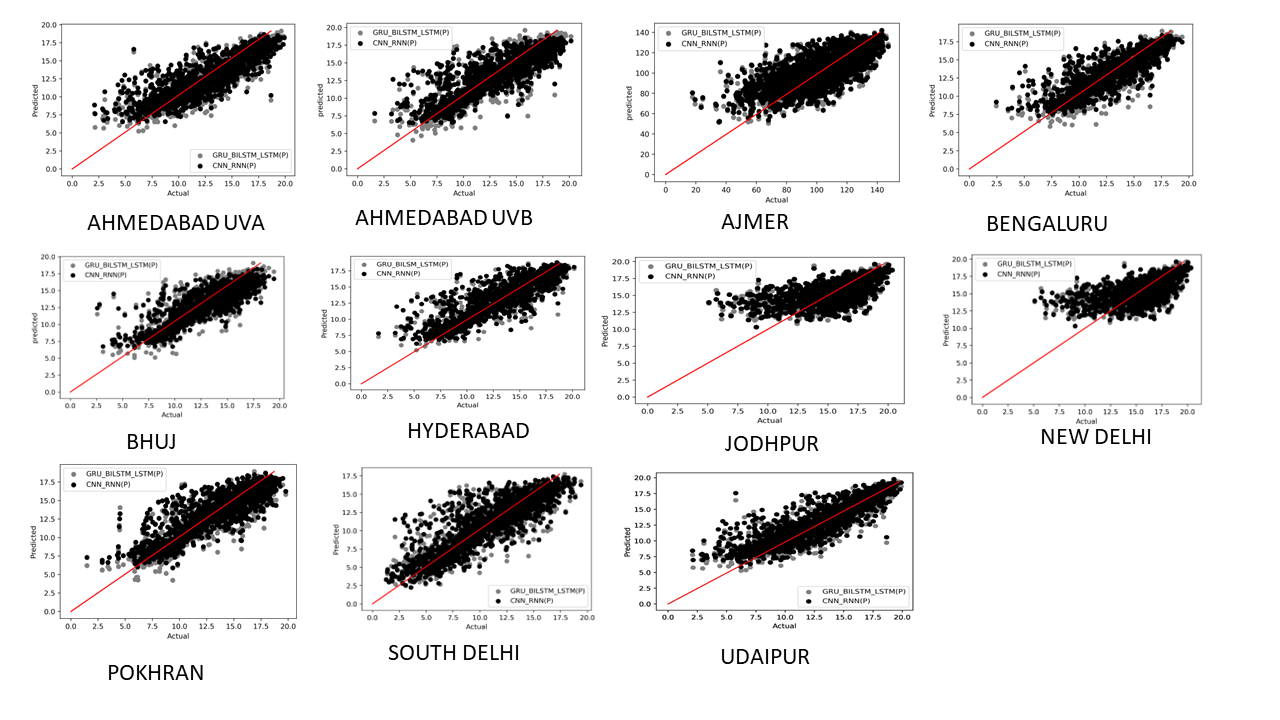
\includegraphics[width=\textwidth]{PROPOSED_SCATTER}
      \caption{Scatter Plot of Proposed Model}
      \label{Line plot1}
      \end{figure}
      
      
      \begin{figure}[!ht]
      \centering
      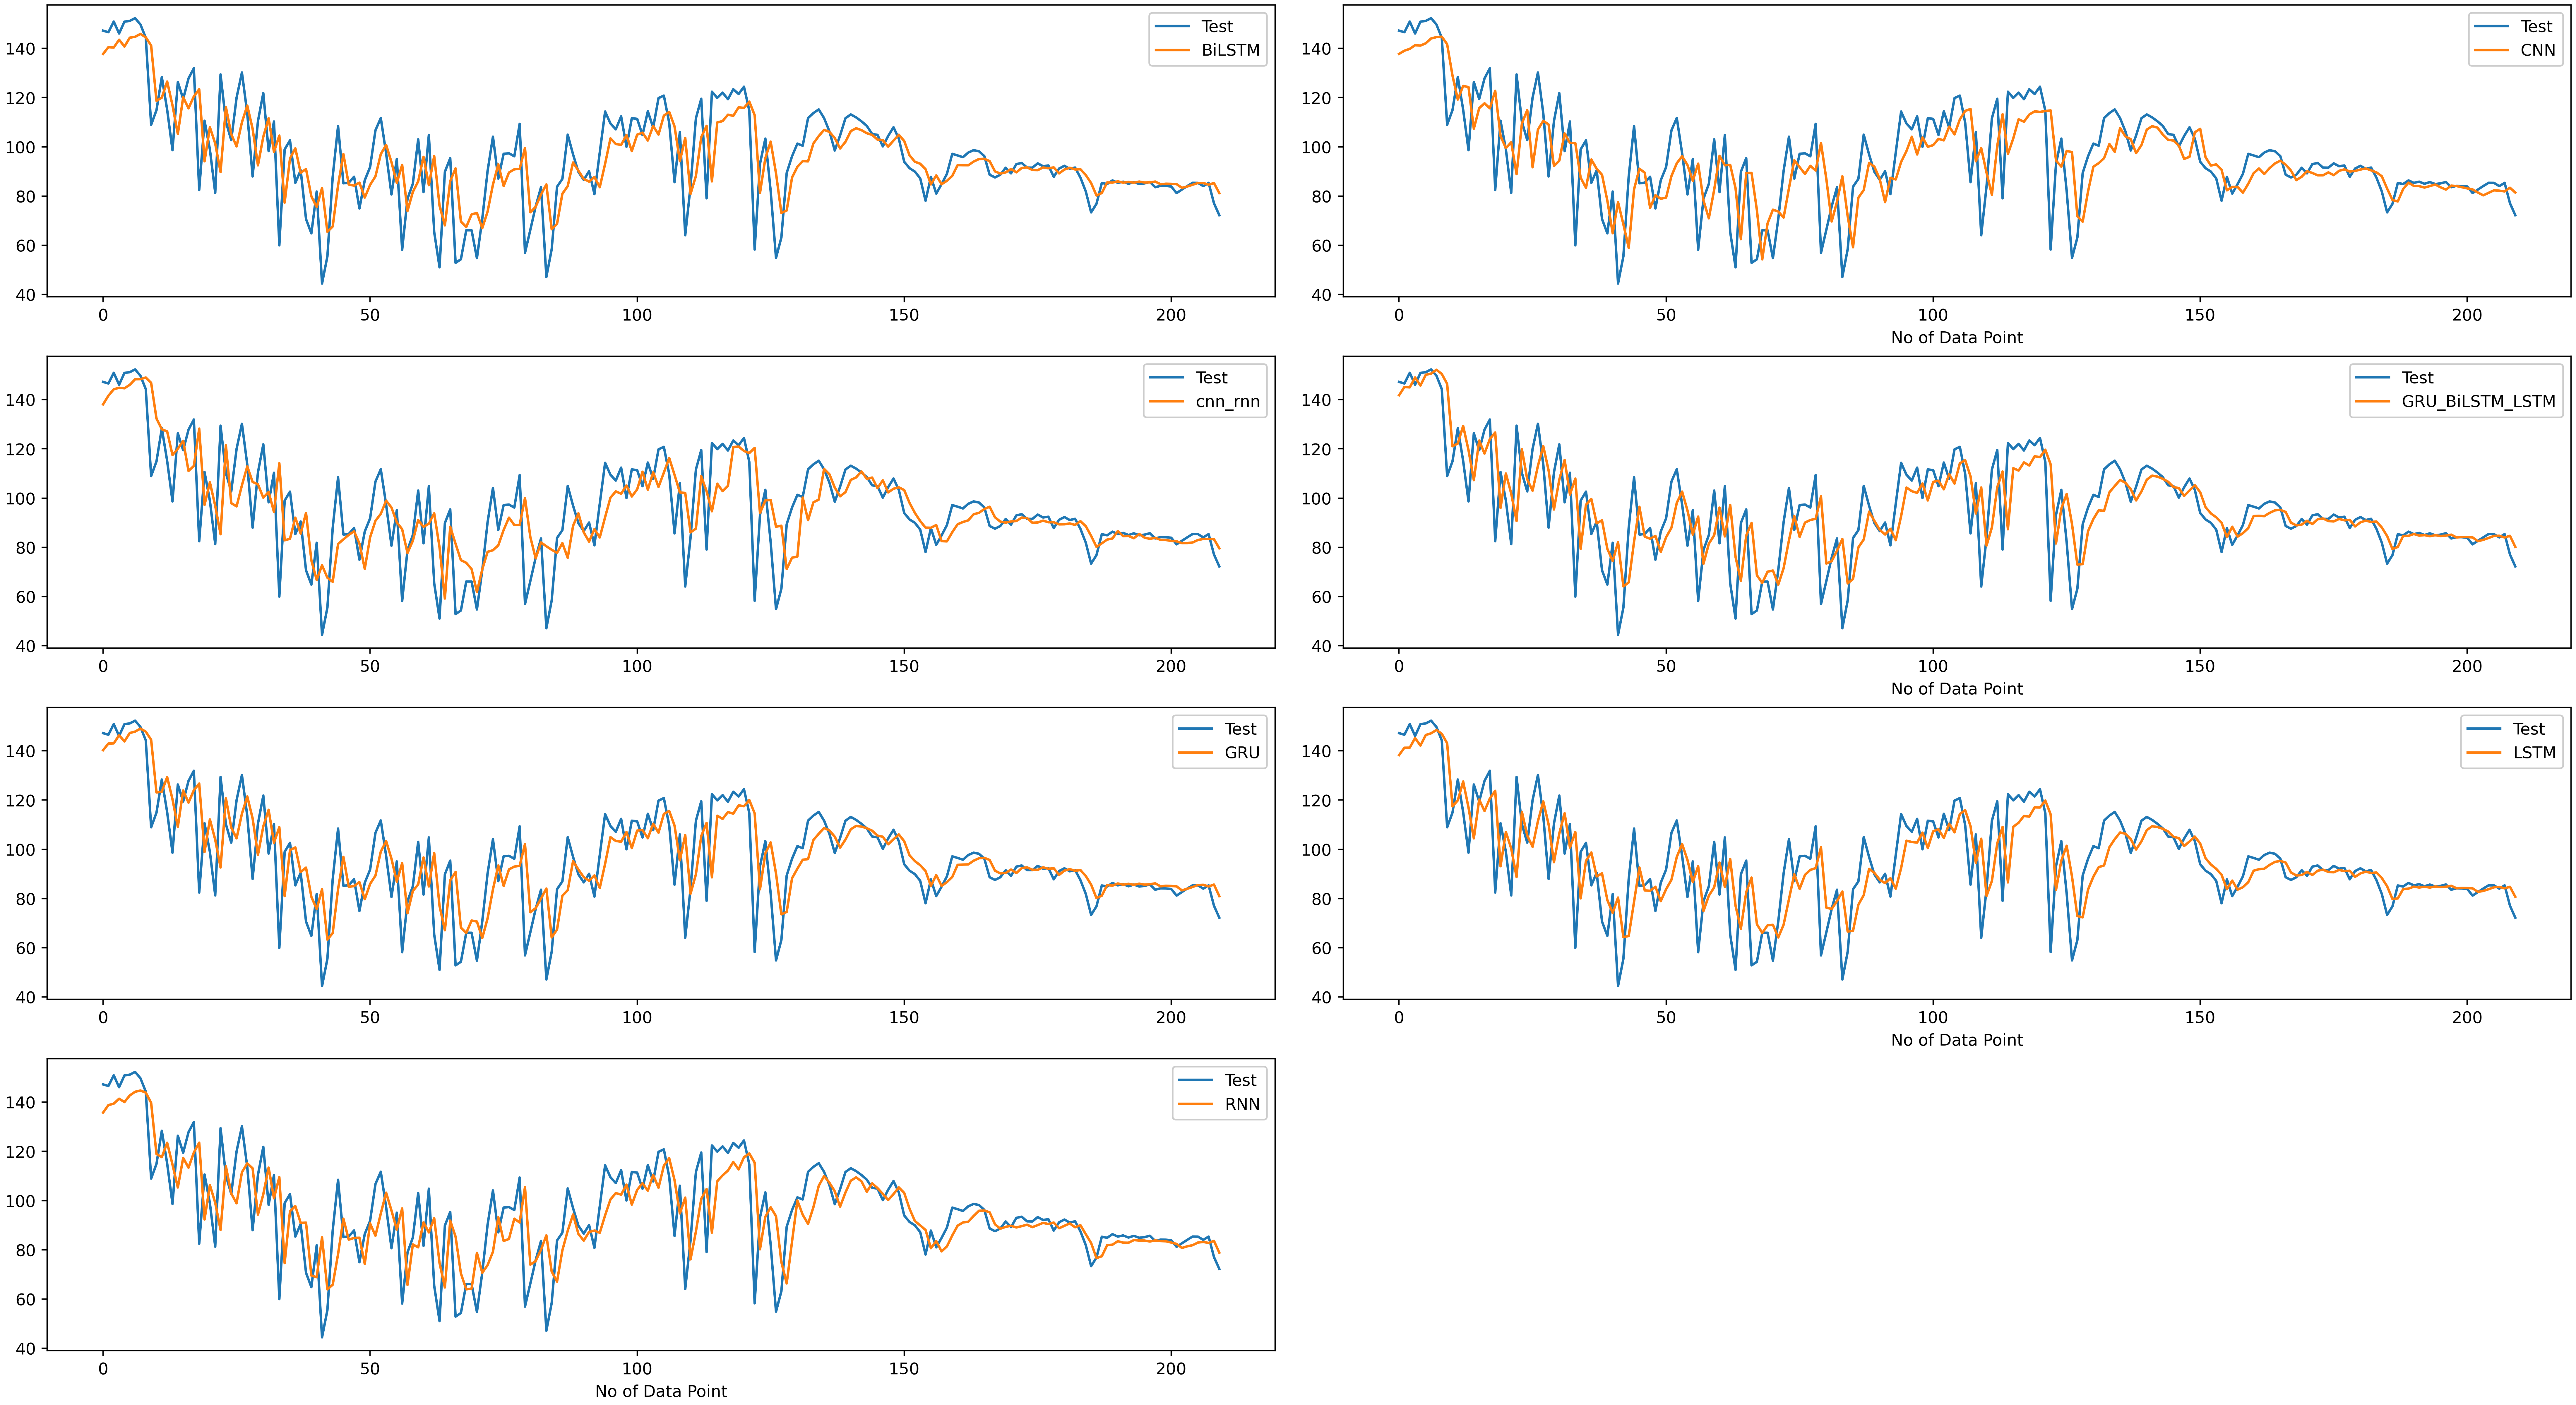
\includegraphics[width=\textwidth]{AHMEDABAD_act vs pred}
      \caption{Line plot Actual vs Prediction}
      \label{Line plot2}
      \end{figure}
      
      
      \begin{figure}[!ht]
      \centering
      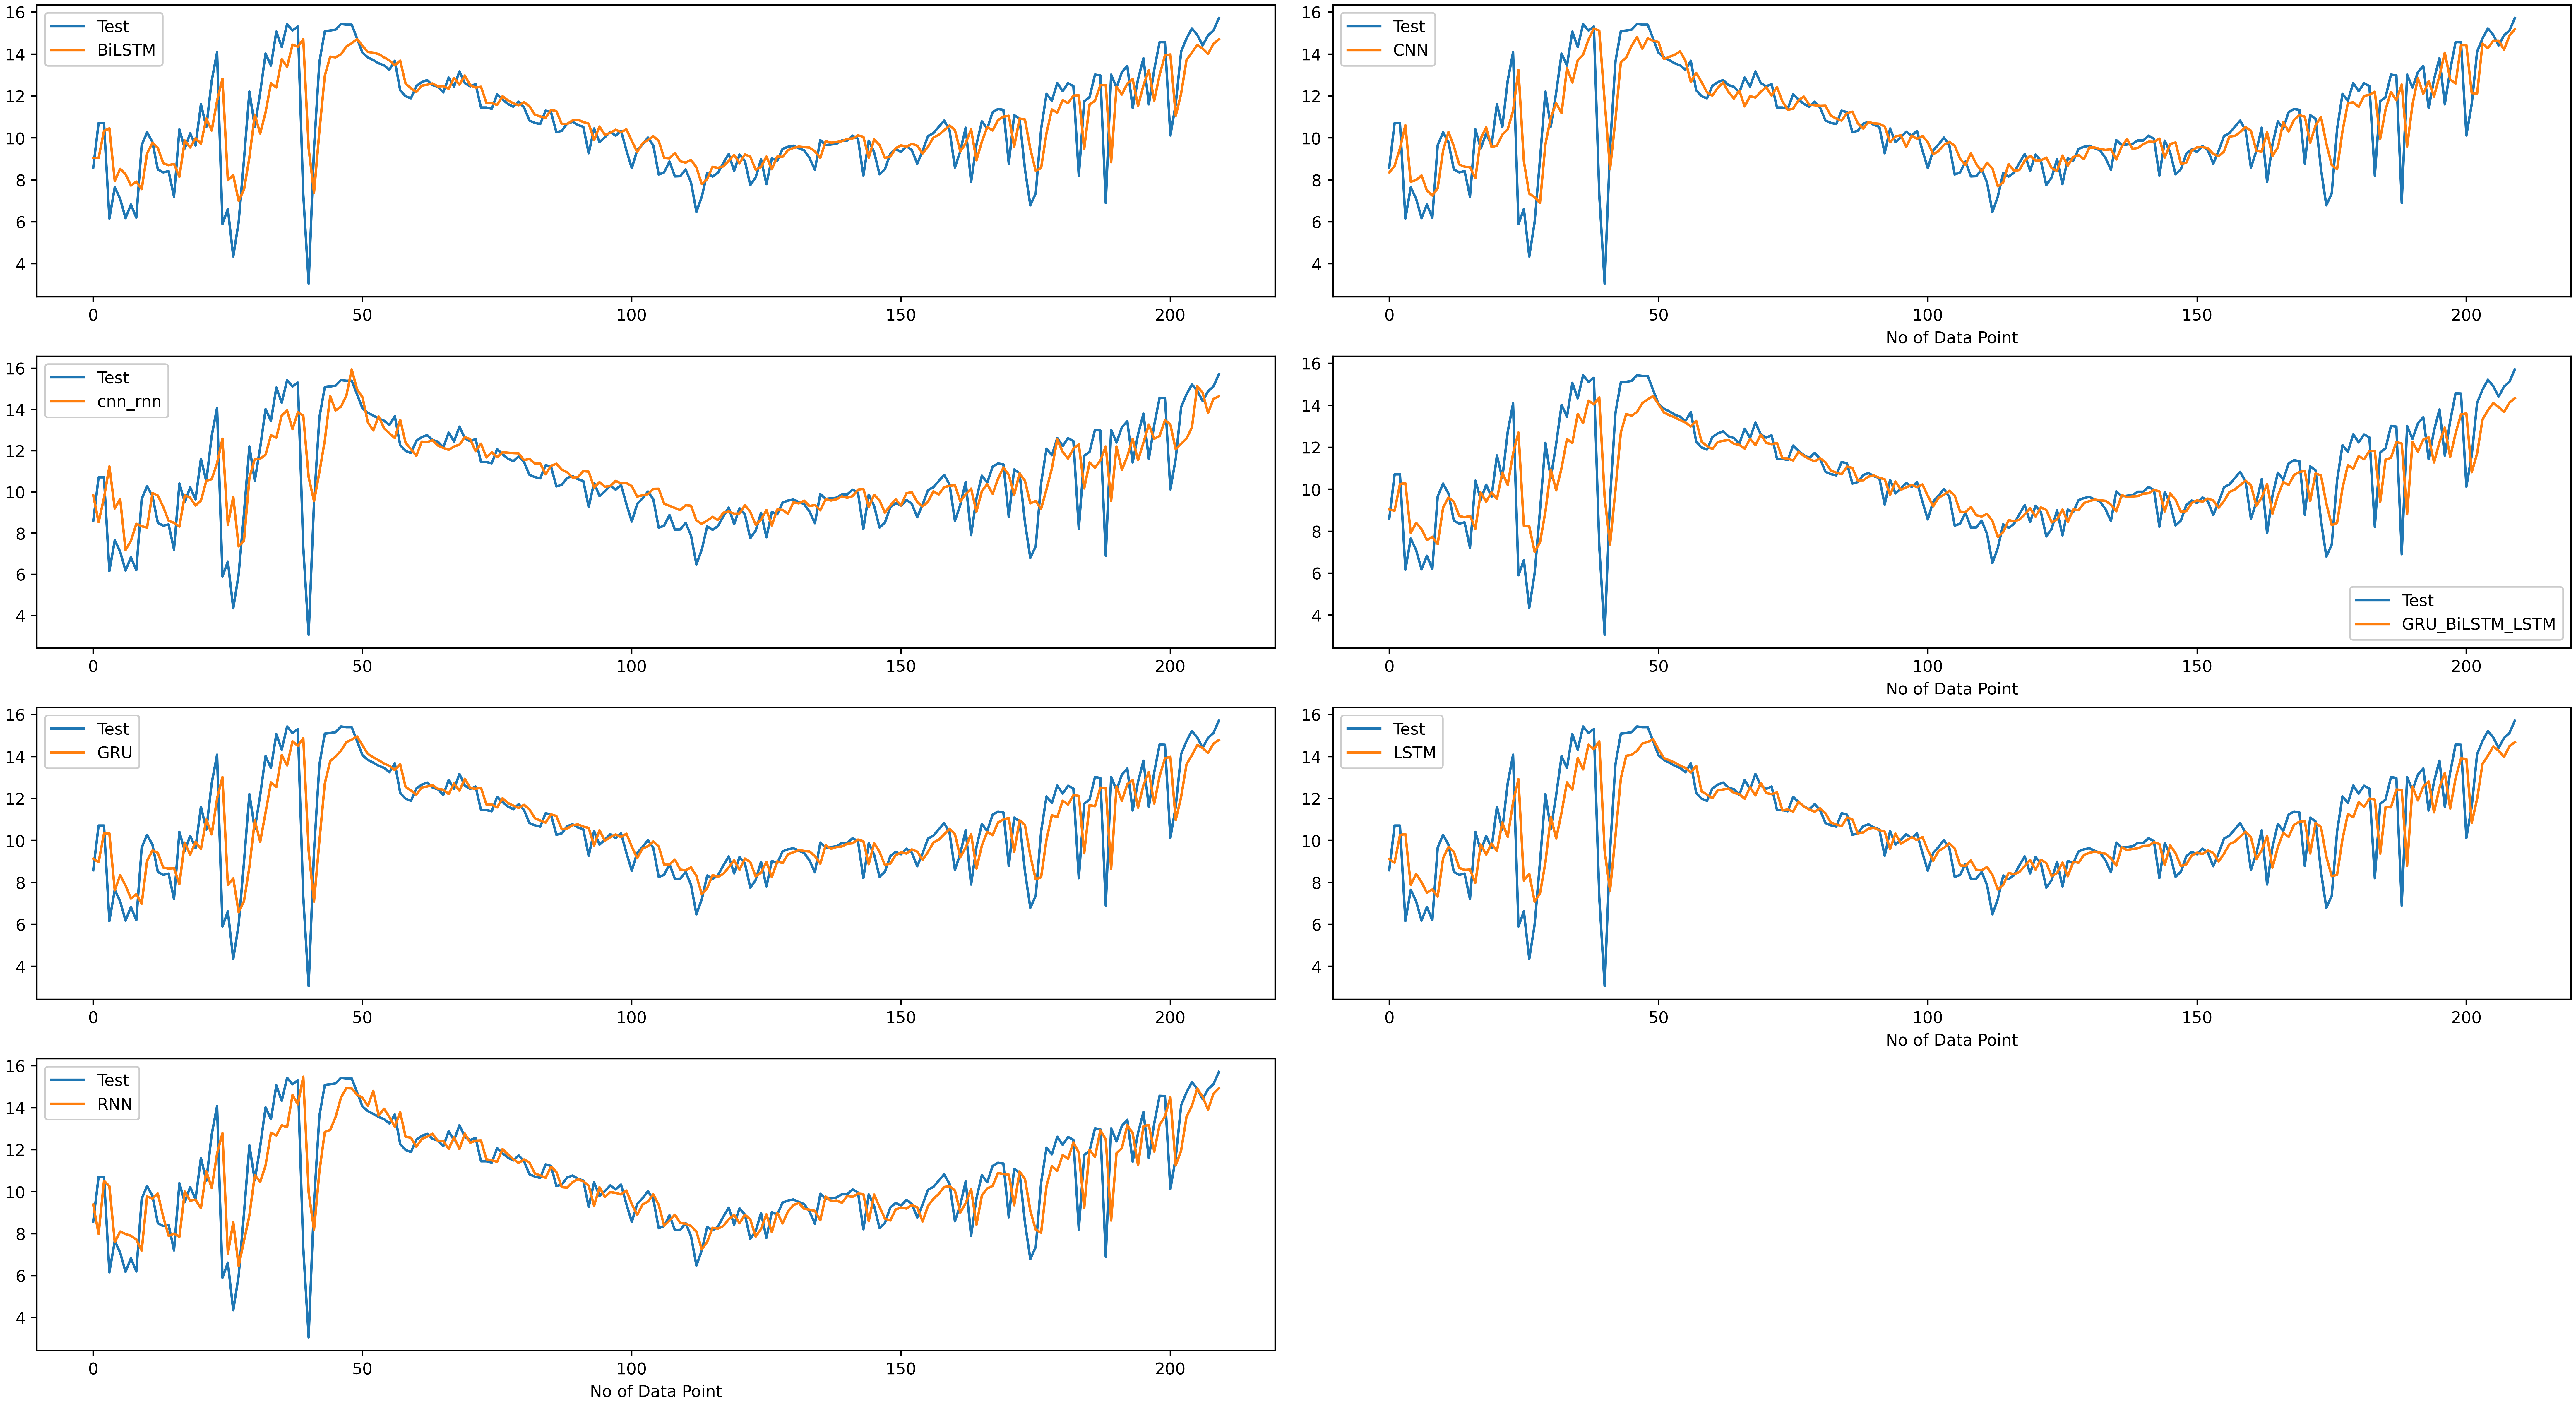
\includegraphics[width=\textwidth]{AHMEDABAD2._act vs pred}
      \caption{Line plot Actual vs Prediction}
      \label{Line plot3}
      \end{figure}
      
      
      \begin{figure}[!ht]
      \centering
      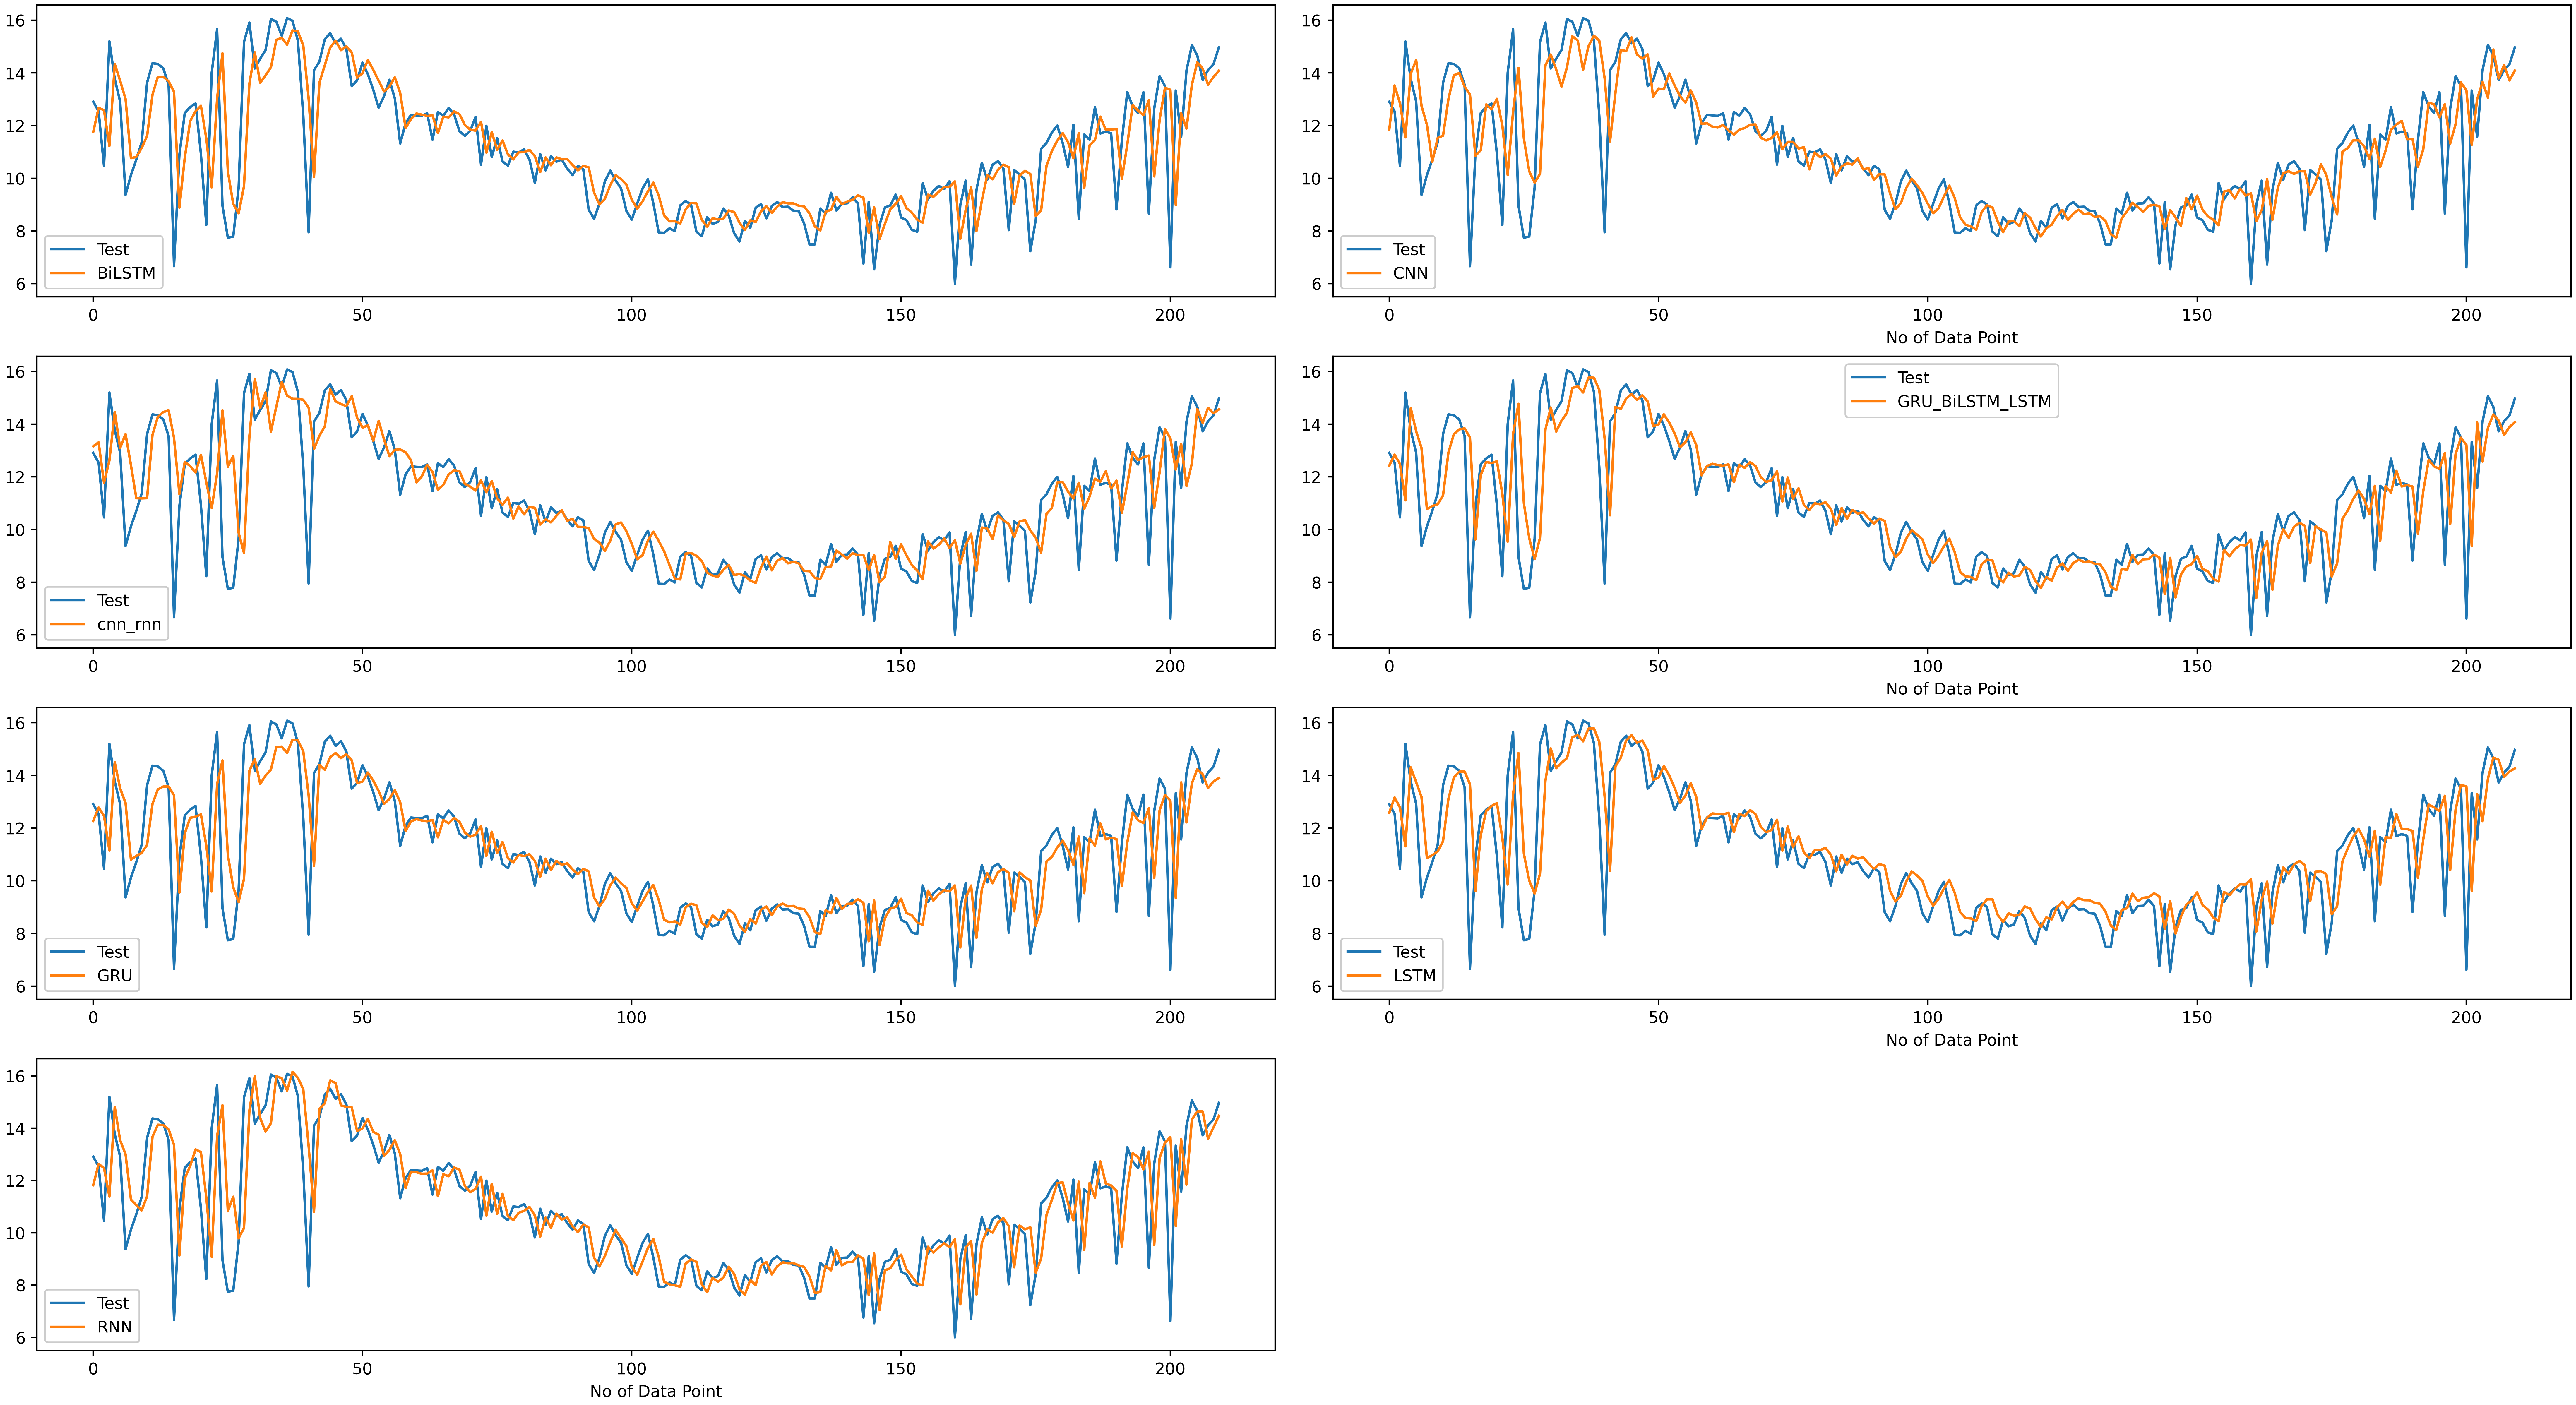
\includegraphics[width=\textwidth]{Ajmer_act vs pred (2)}
      \caption{Line plot Actual vs Prediction}
      \label{Line plot4}
      \end{figure}
      
      
      
      \begin{figure}[!ht]
      \centering
      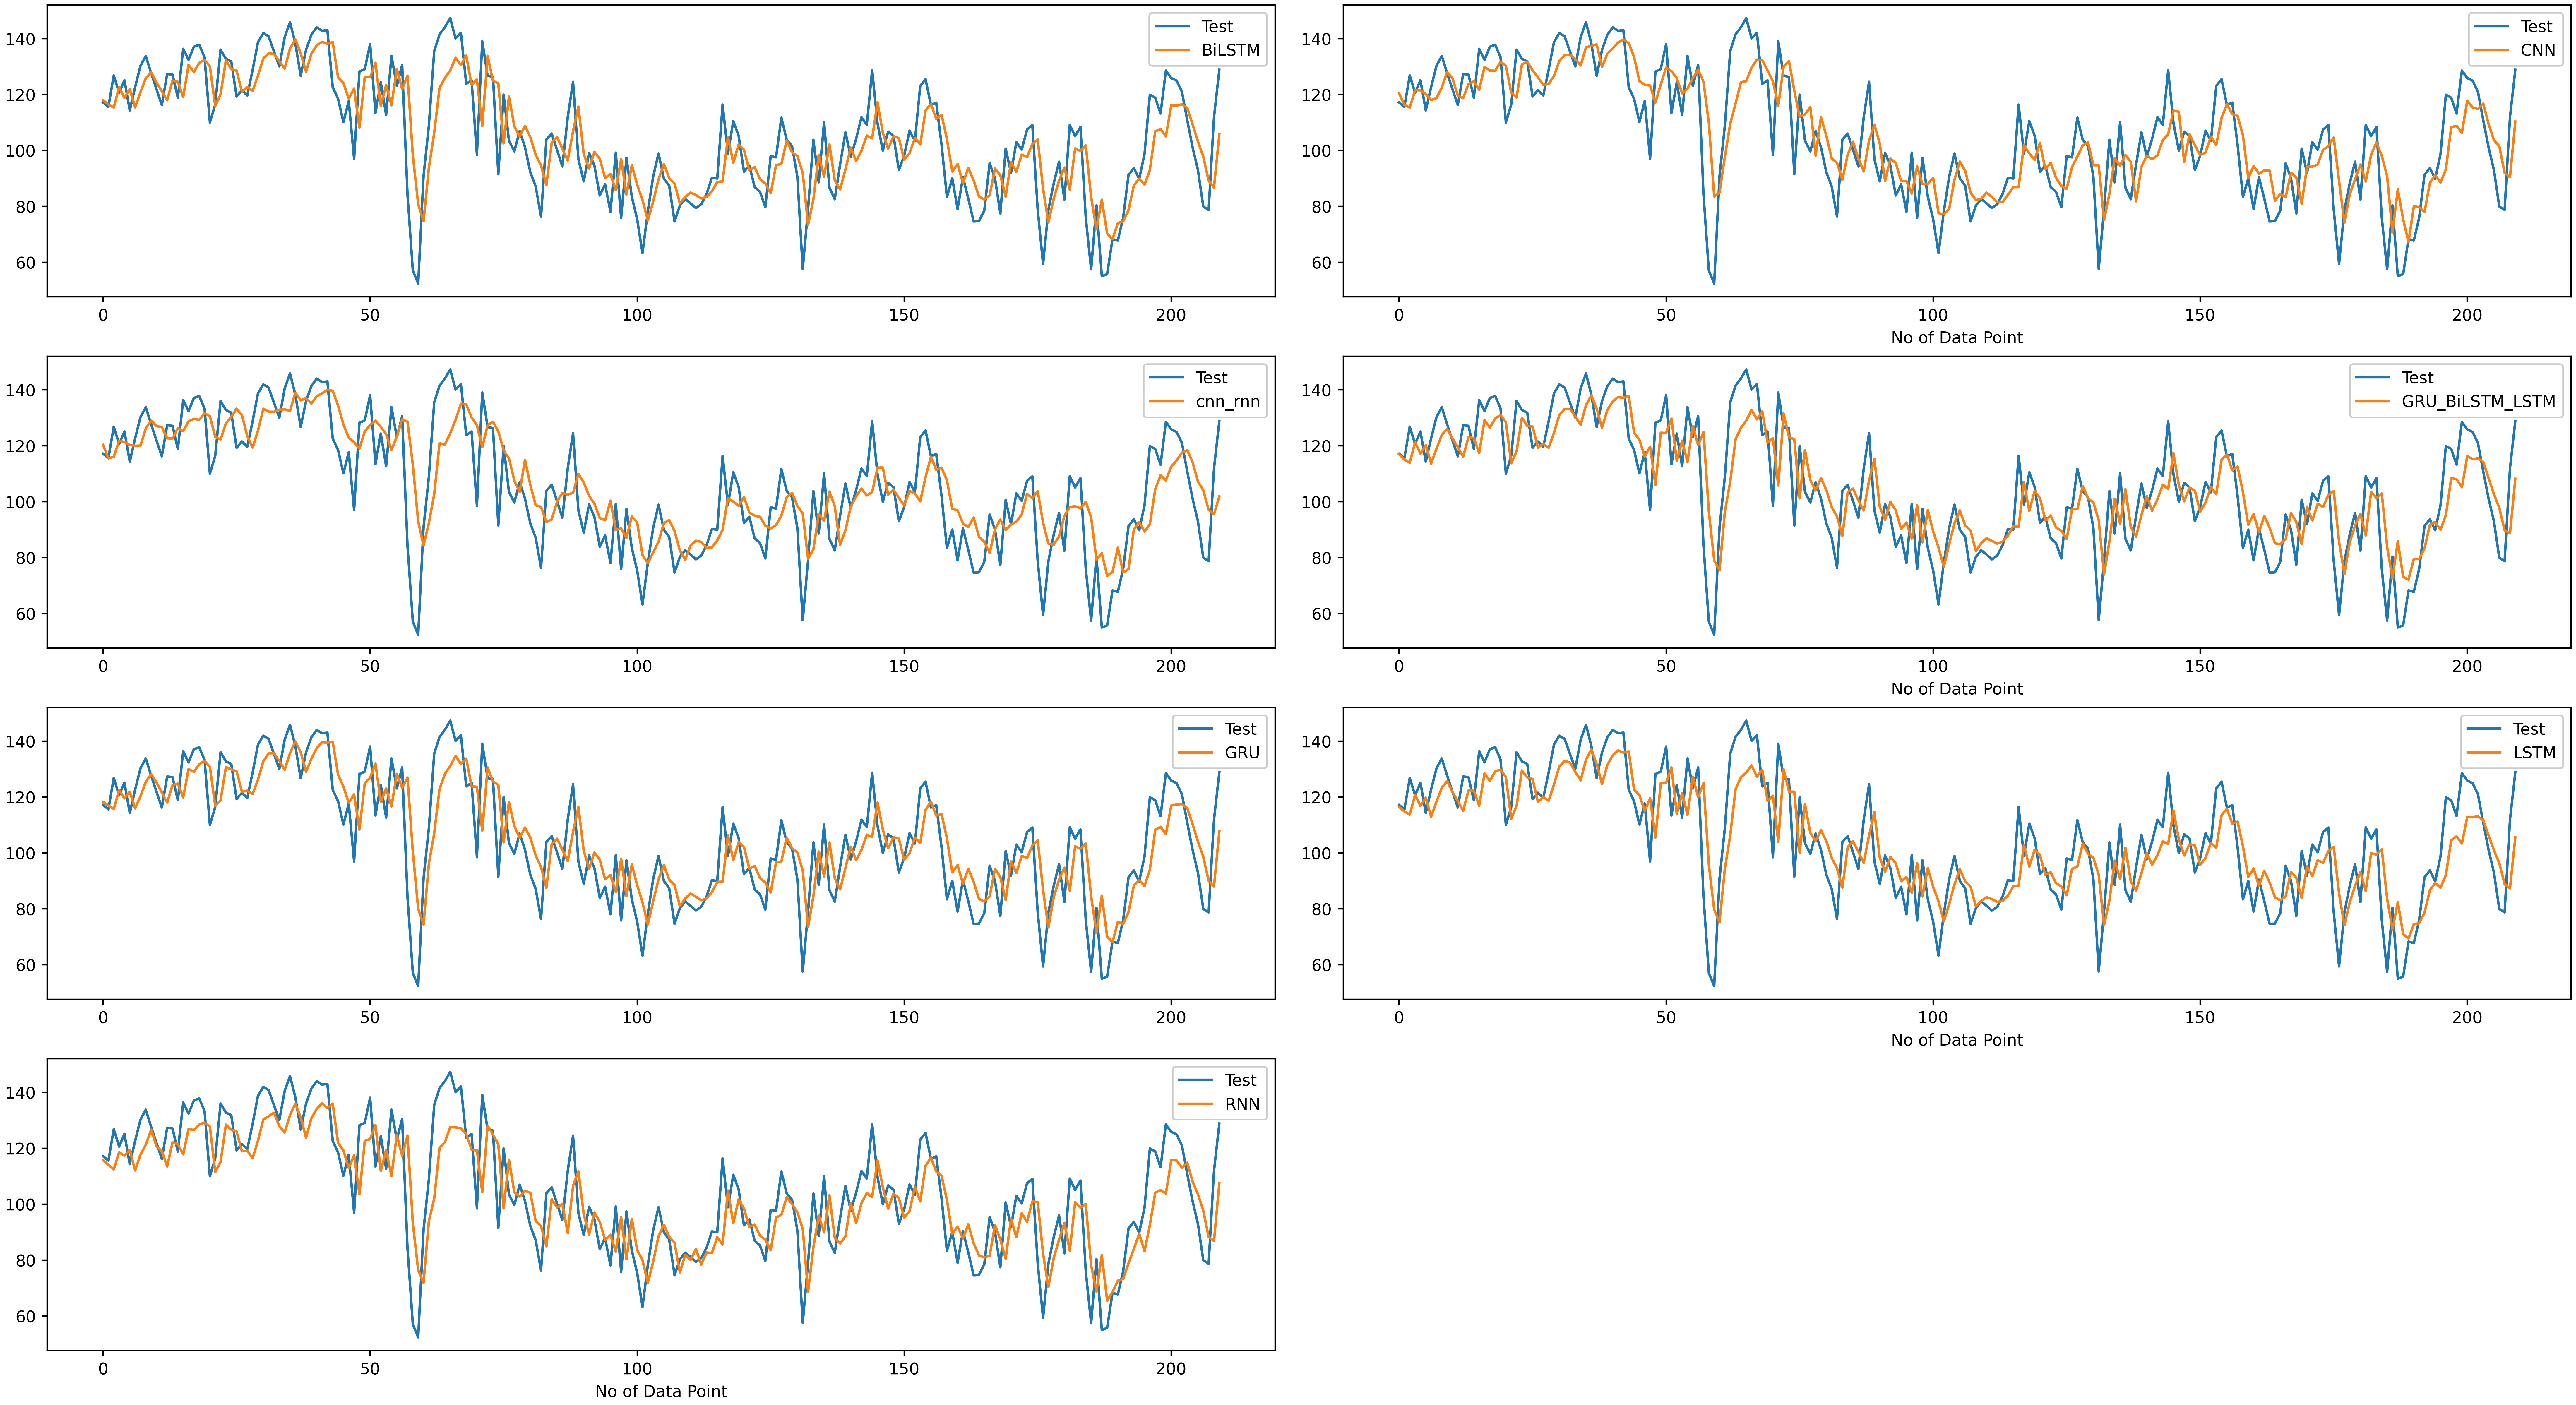
\includegraphics[width=\textwidth]{Bengaluru_act vs pred}
      \caption{Line plot Actual vs Prediction}
      \label{Line plot5}
      \end{figure}
      
      
      \begin{figure}[!ht]
      \centering
      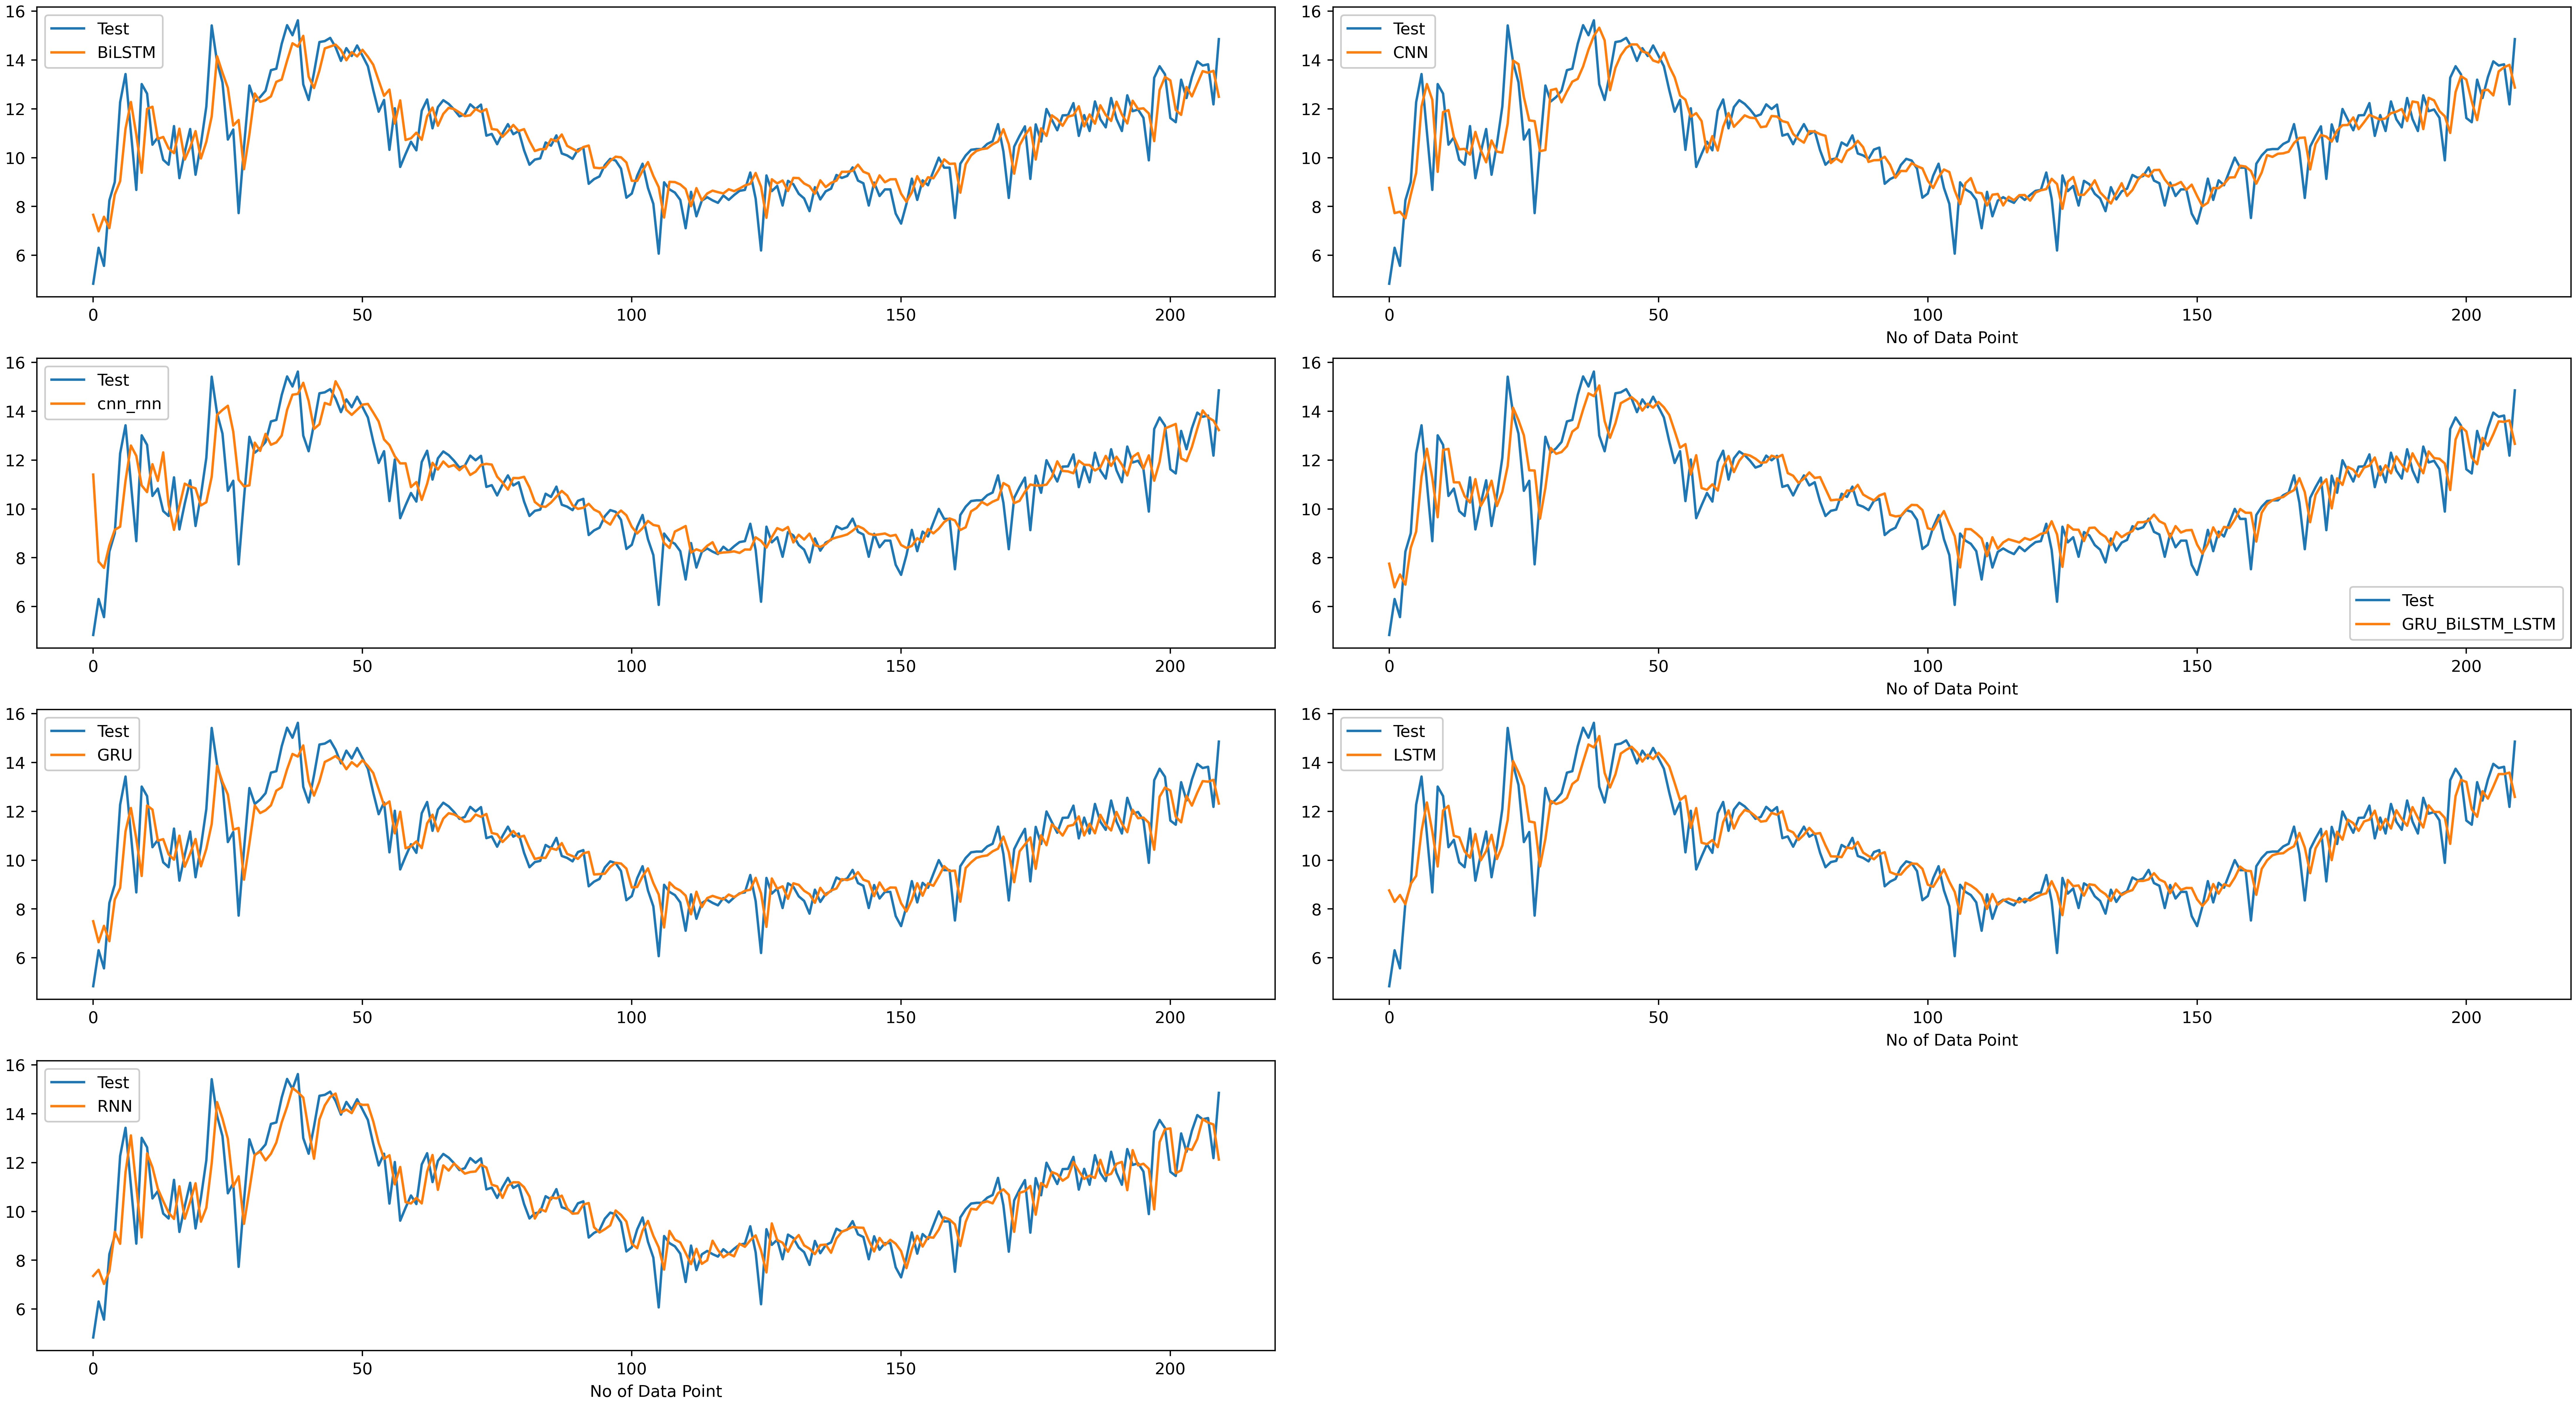
\includegraphics[width=\textwidth]{Bhuj_act vs pred}
      \caption{Line Plot of Proposed Model}
      \label{Line plot6}
      \end{figure}
      
      
      
      \begin{figure}[!ht]
      \centering
      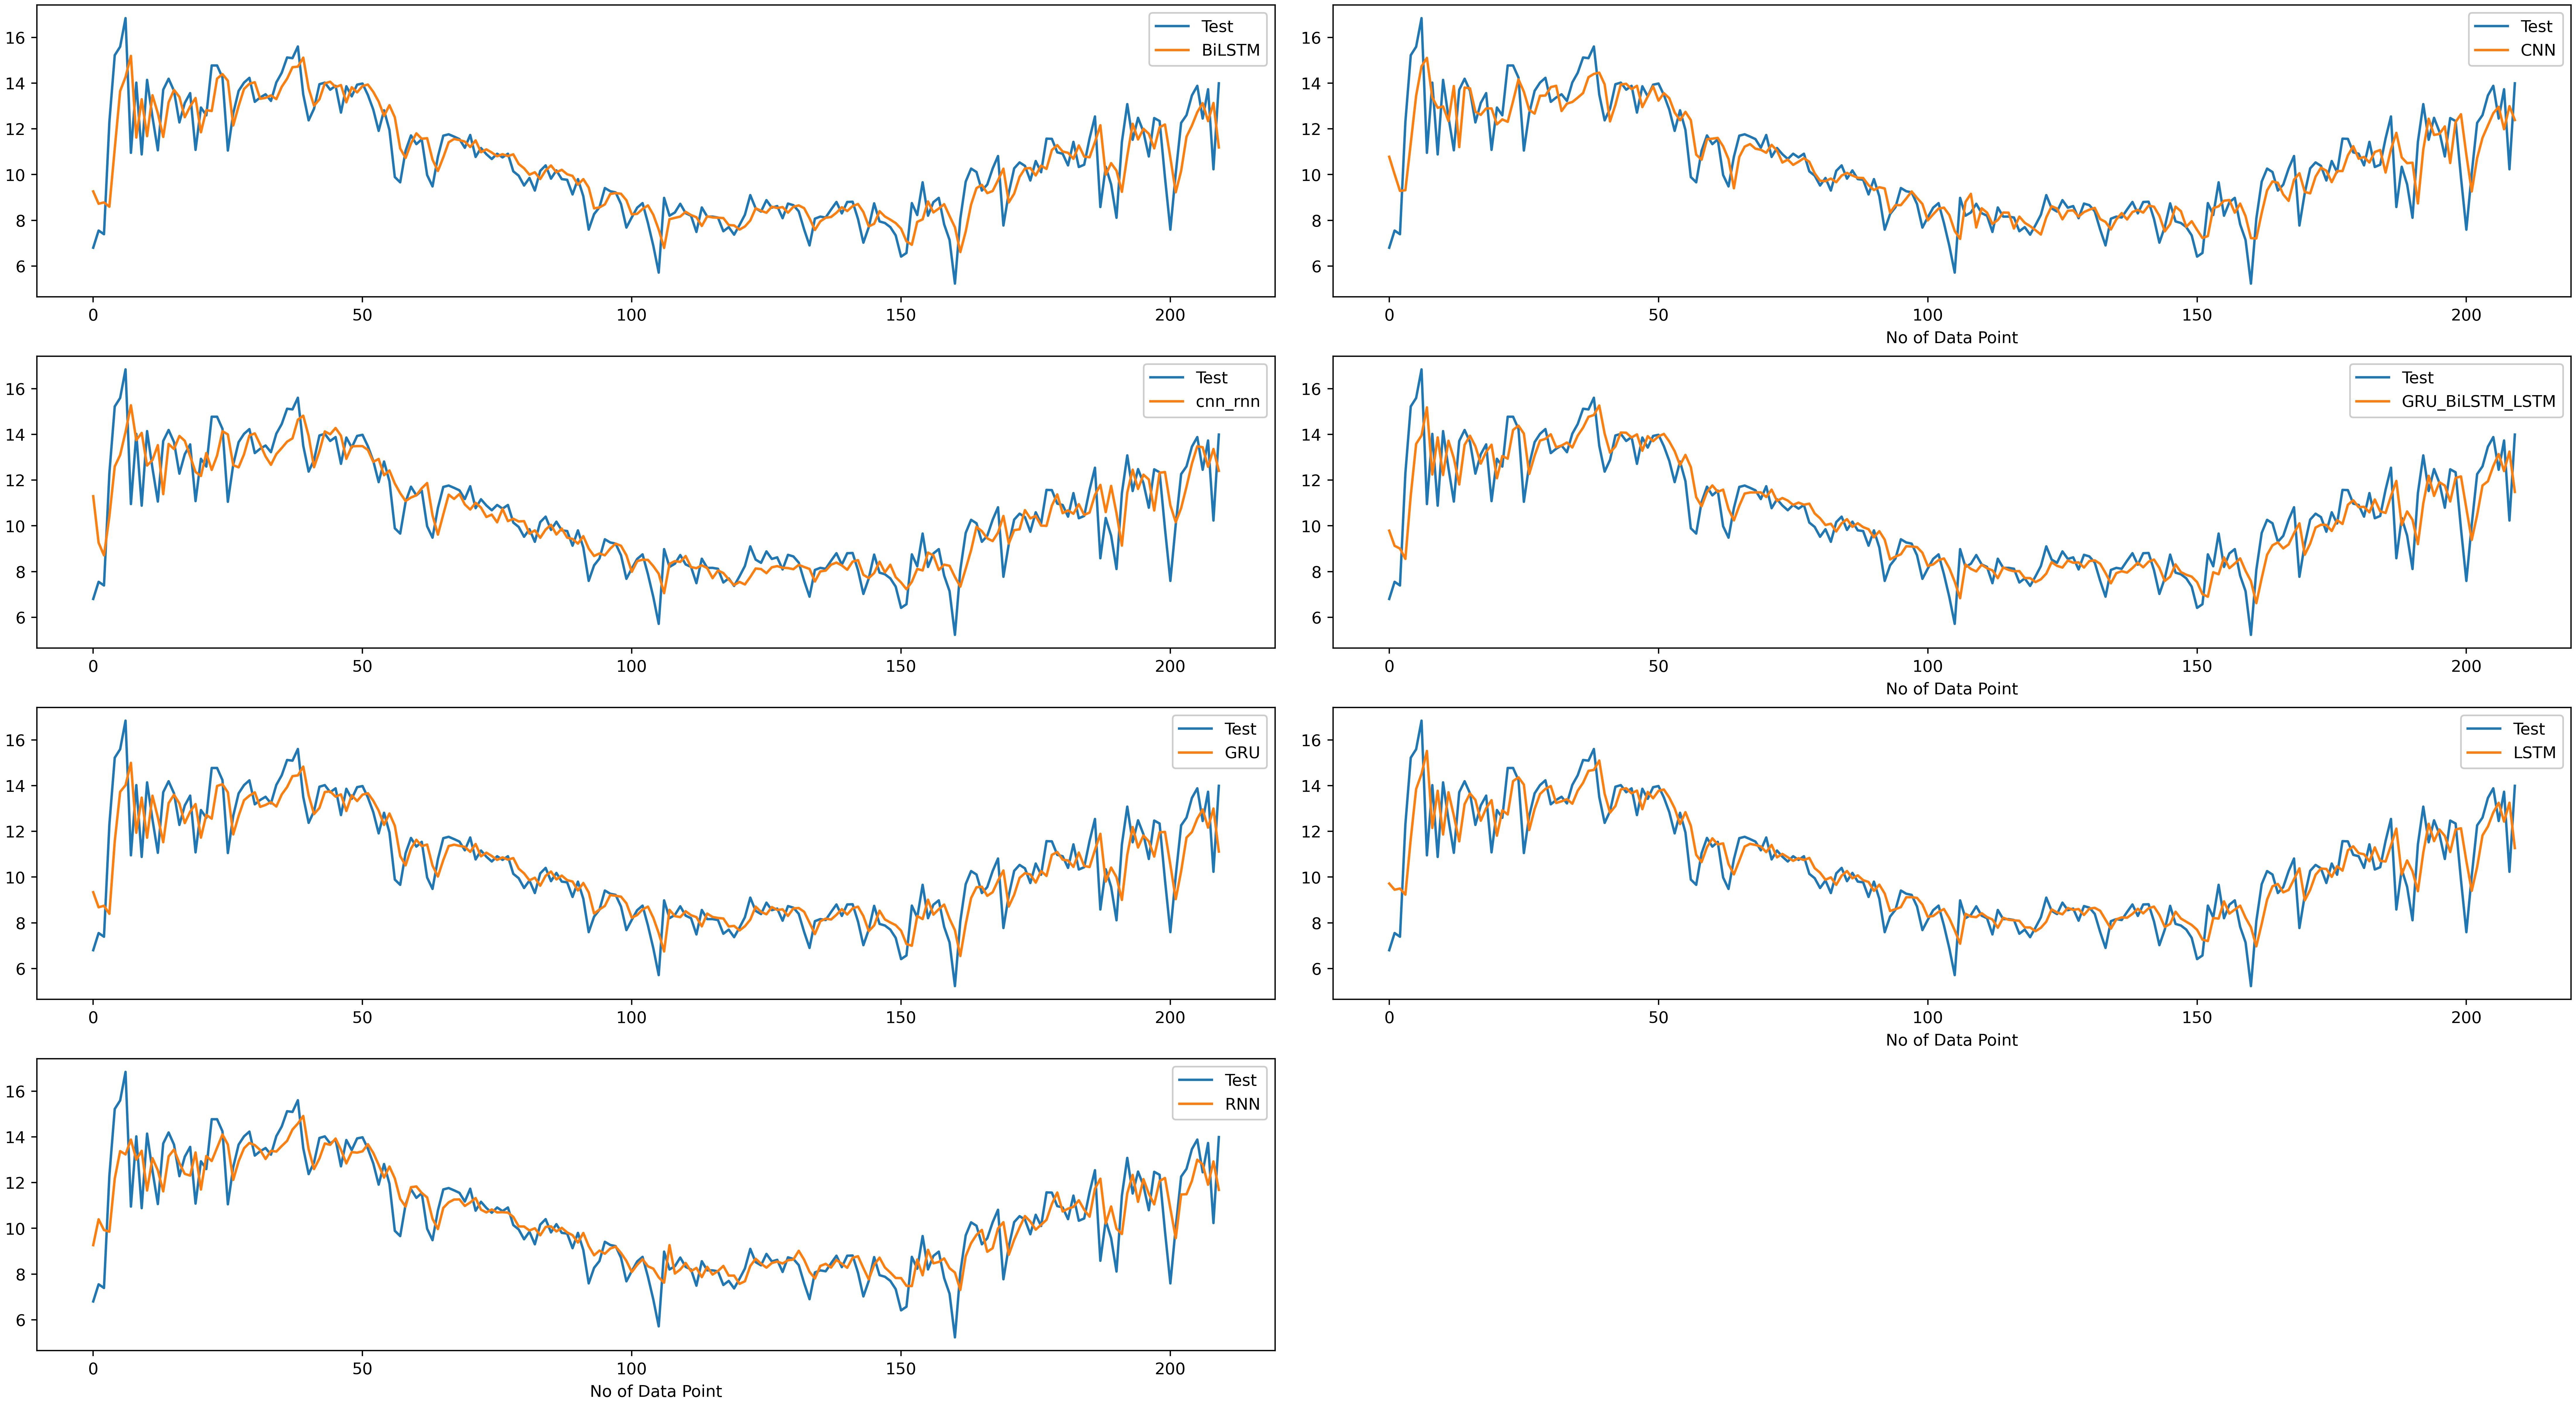
\includegraphics[width=\textwidth]{hyderabad_act vs pred}
      \caption{Line plot Actual vs Predictionl}
      \label{Line plot7}
      \end{figure}
      
      
      
      \begin{figure}[!ht]
      \centering
      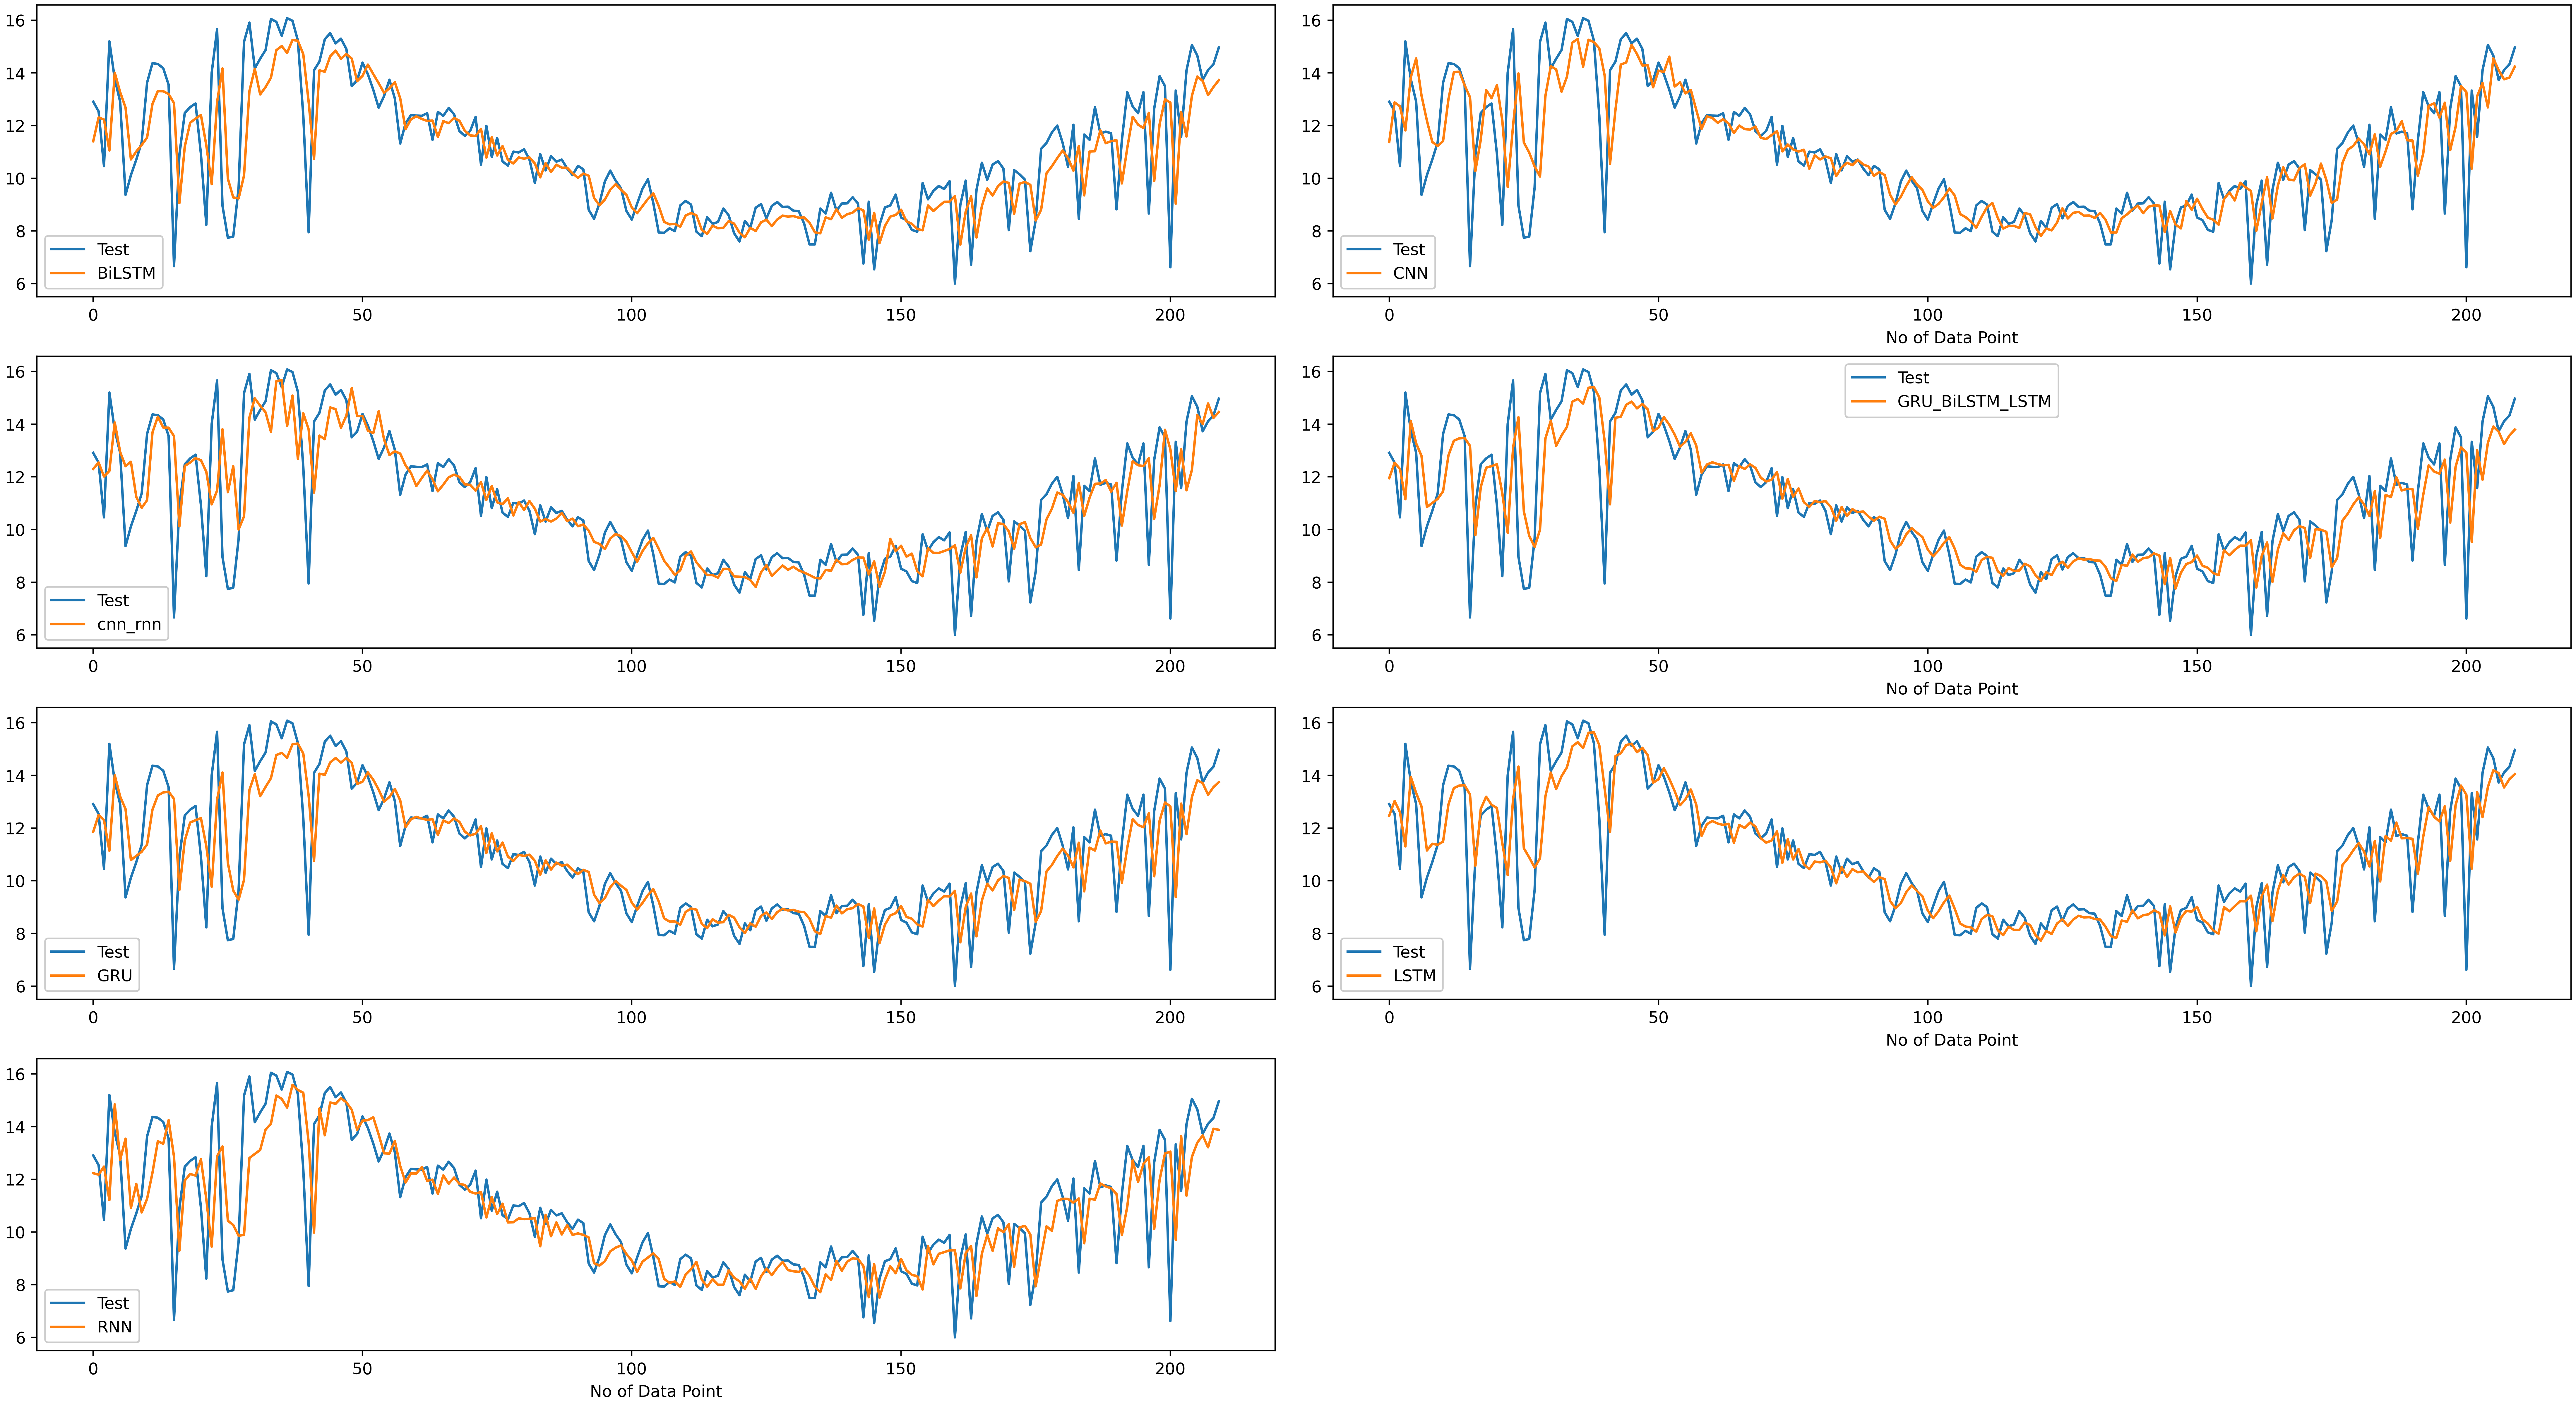
\includegraphics[width=\textwidth]{Jodhpur (2)_act vs pred}
      \caption{Line plot Actual vs Prediction}
      \label{Line plot8}
      \end{figure}
      
      
      \begin{figure}[!ht]
      \centering
      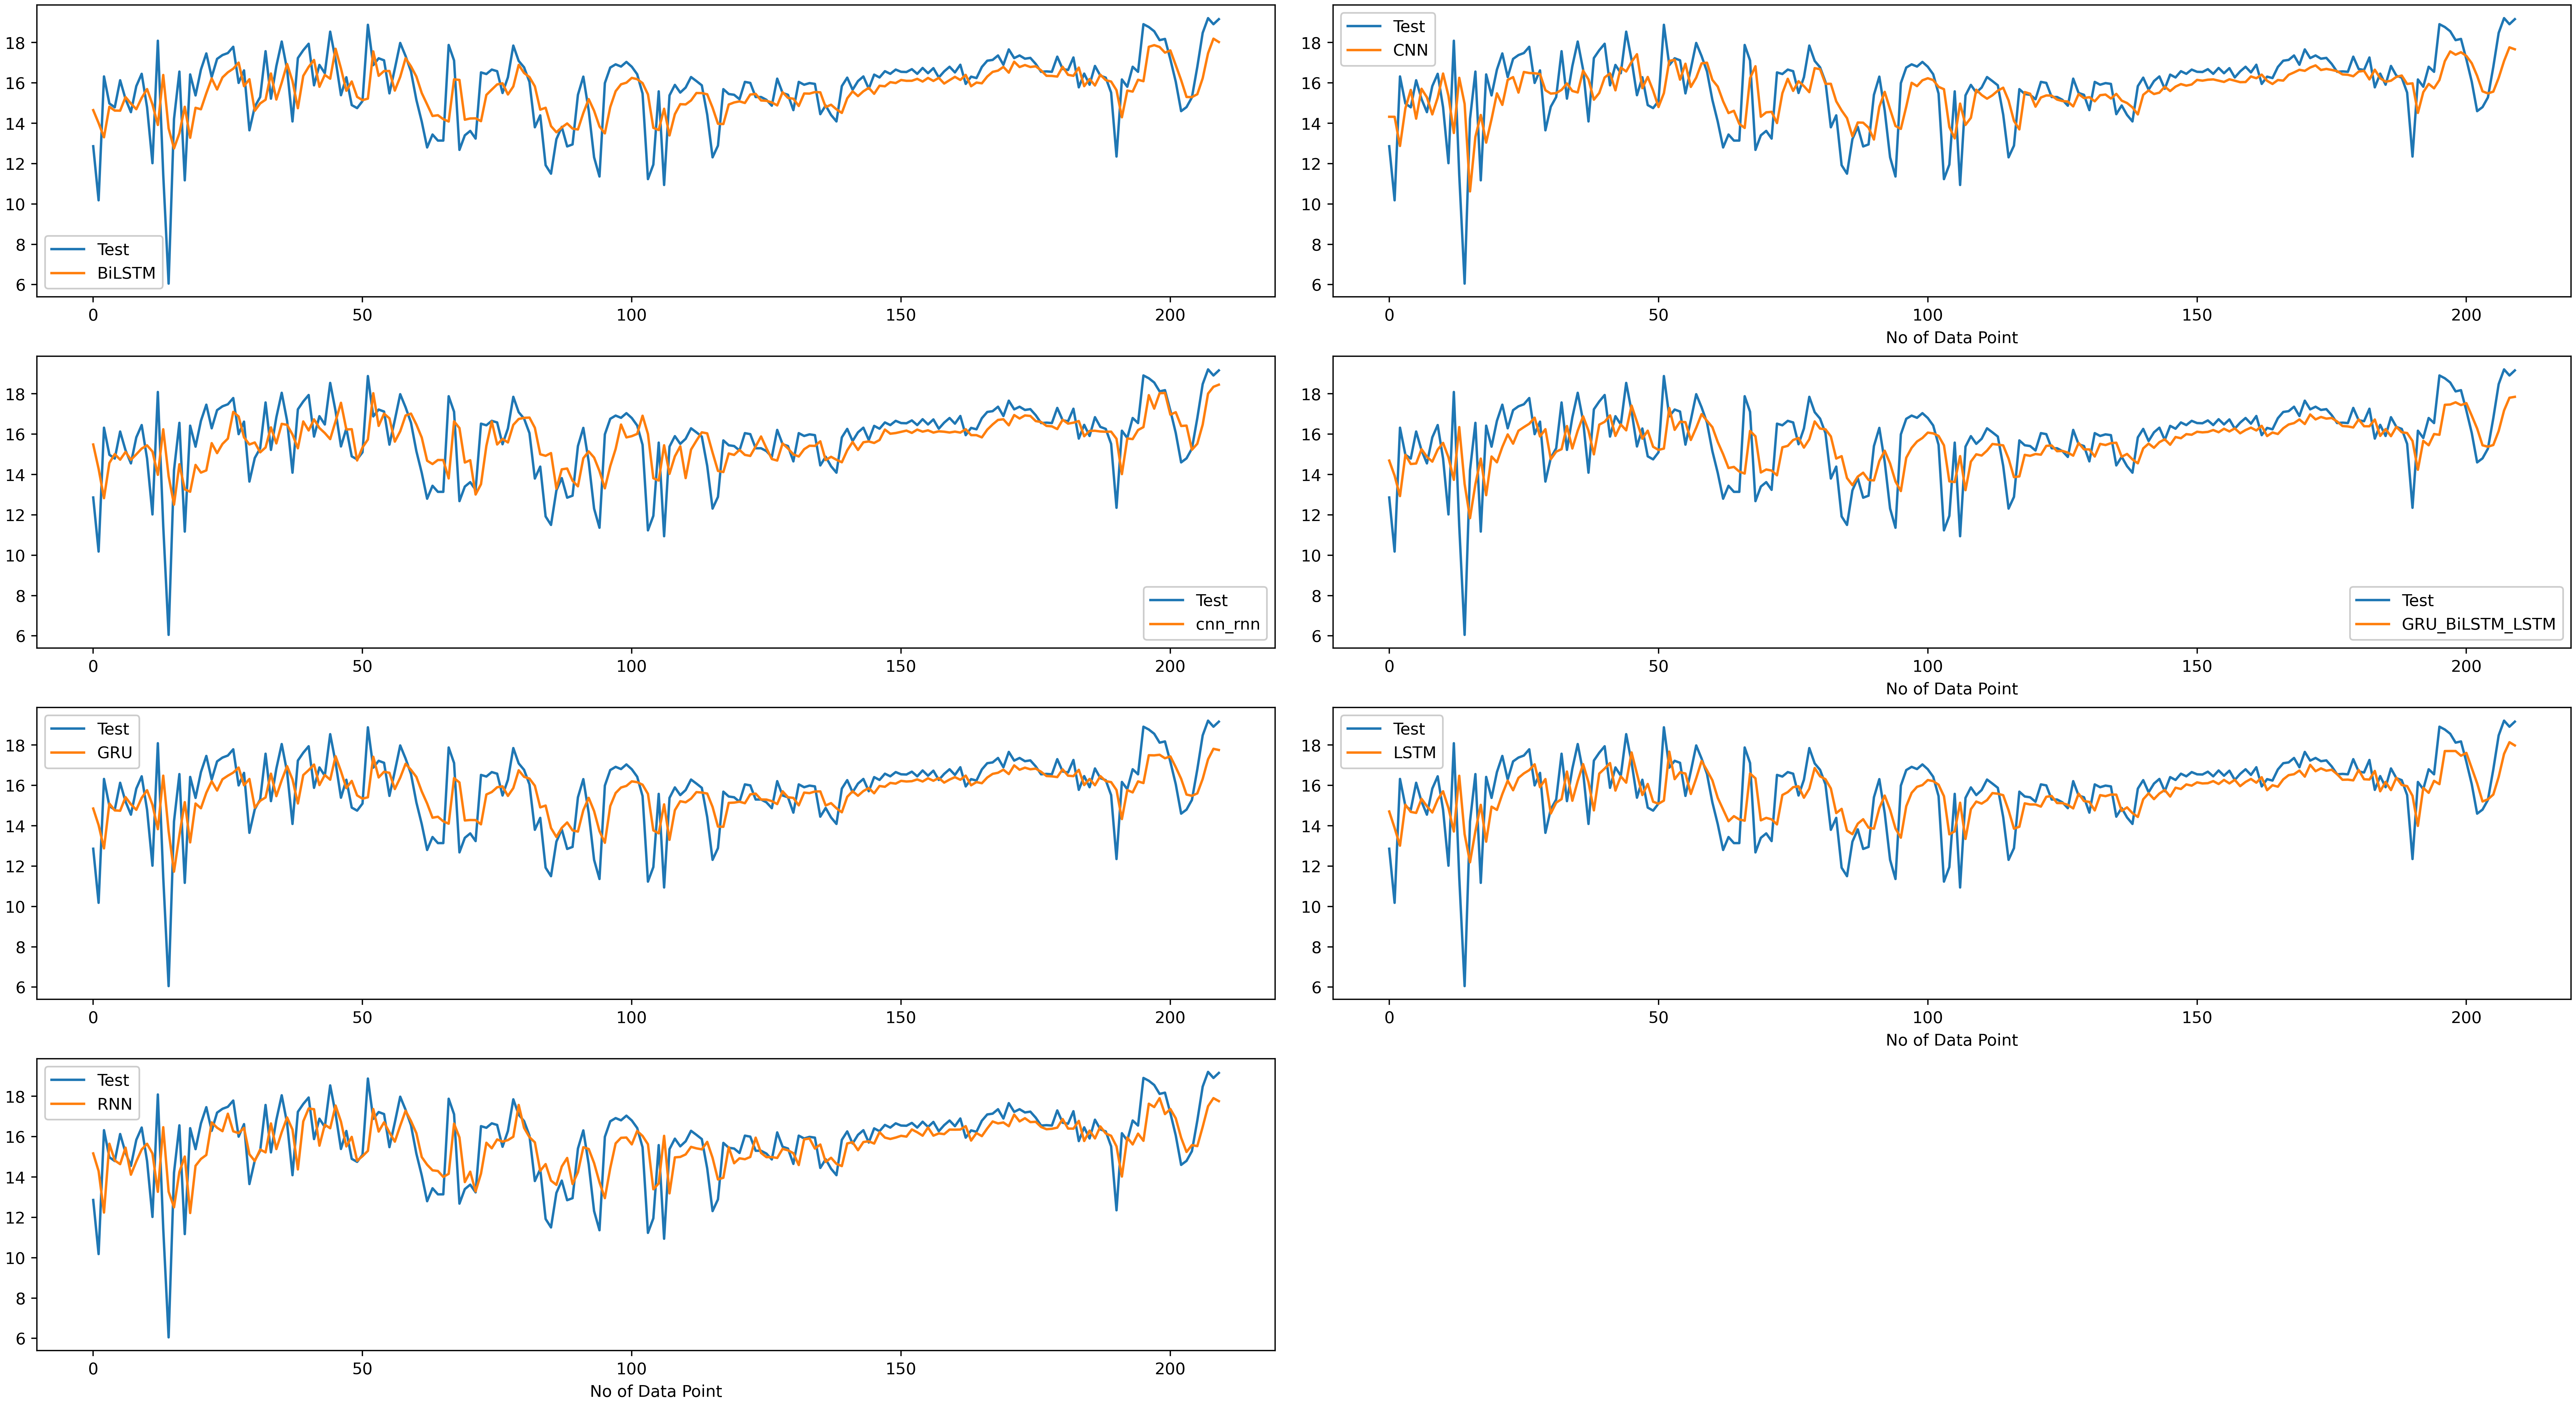
\includegraphics[width=\textwidth]{new delhi_act vs pred}
      \caption{Line plot Actual vs Prediction}
      \label{Line plot9}
      \end{figure}
      
      
      \begin{figure}[!ht]
      \centering
      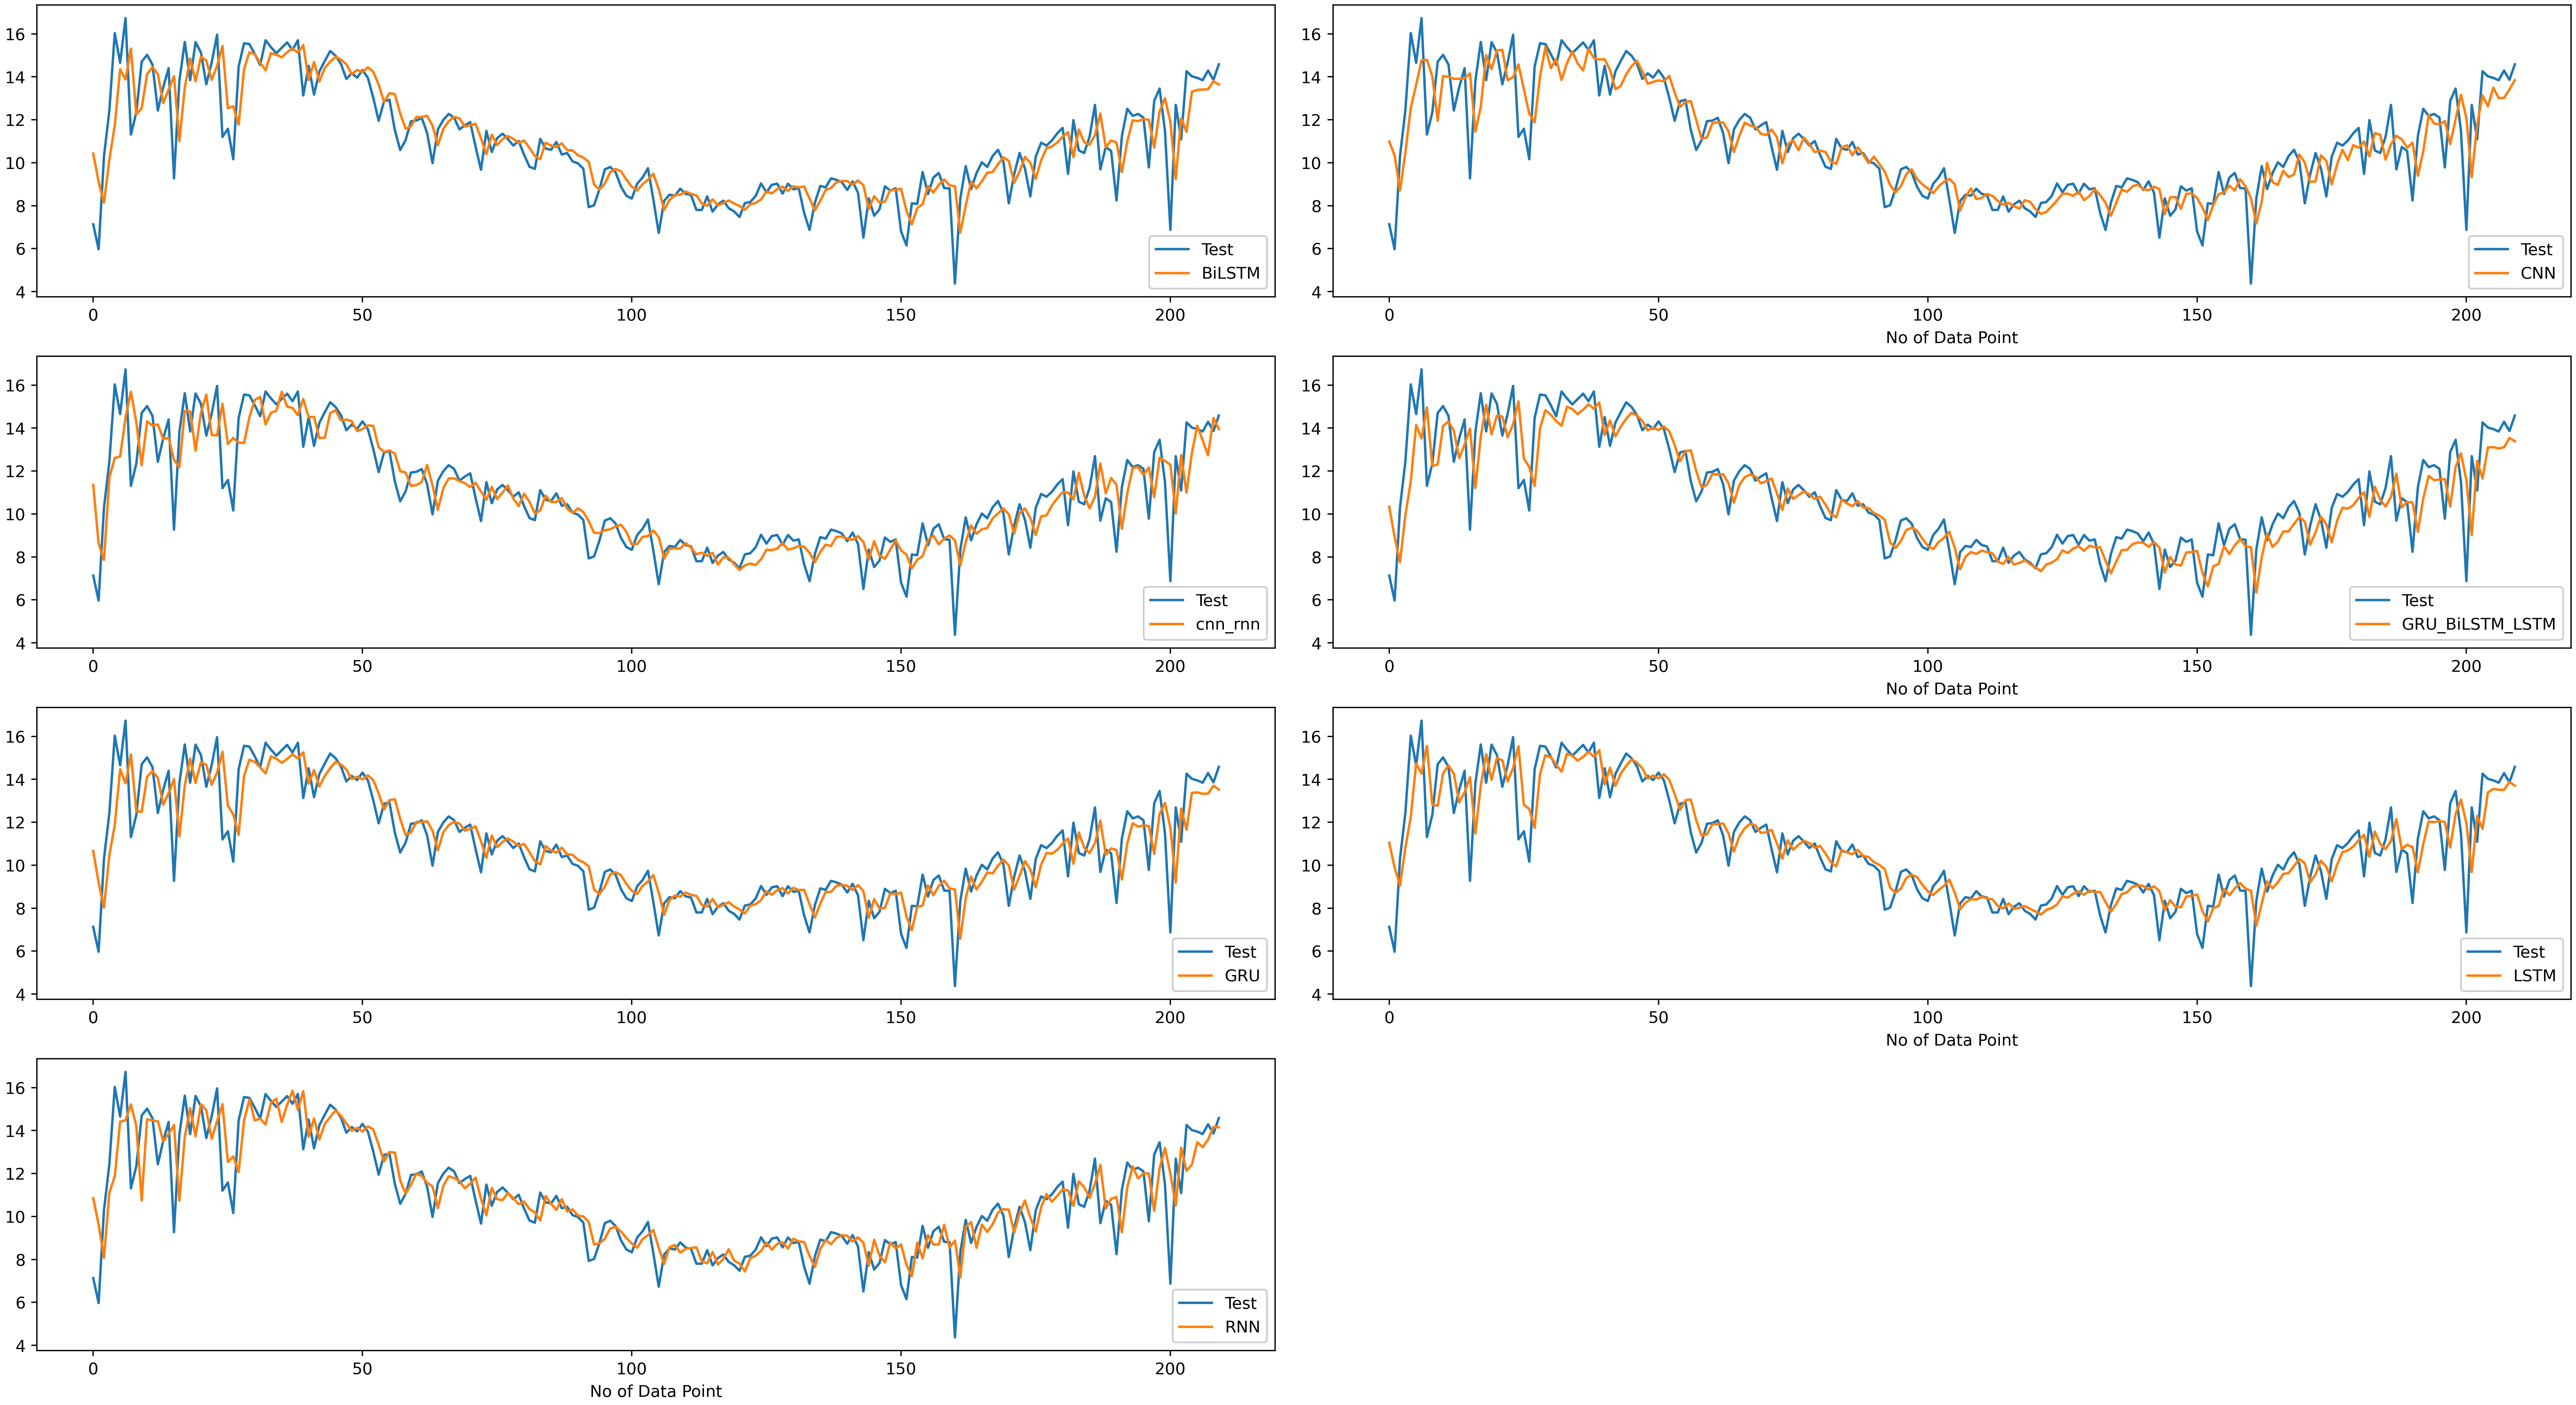
\includegraphics[width=\textwidth]{Pokhran_act vs pred (1)}
      \caption{Line plot Actual vs Prediction}
      \label{fig:plot}
      \end{figure}
      
      \begin{figure}[!ht]
      \centering
      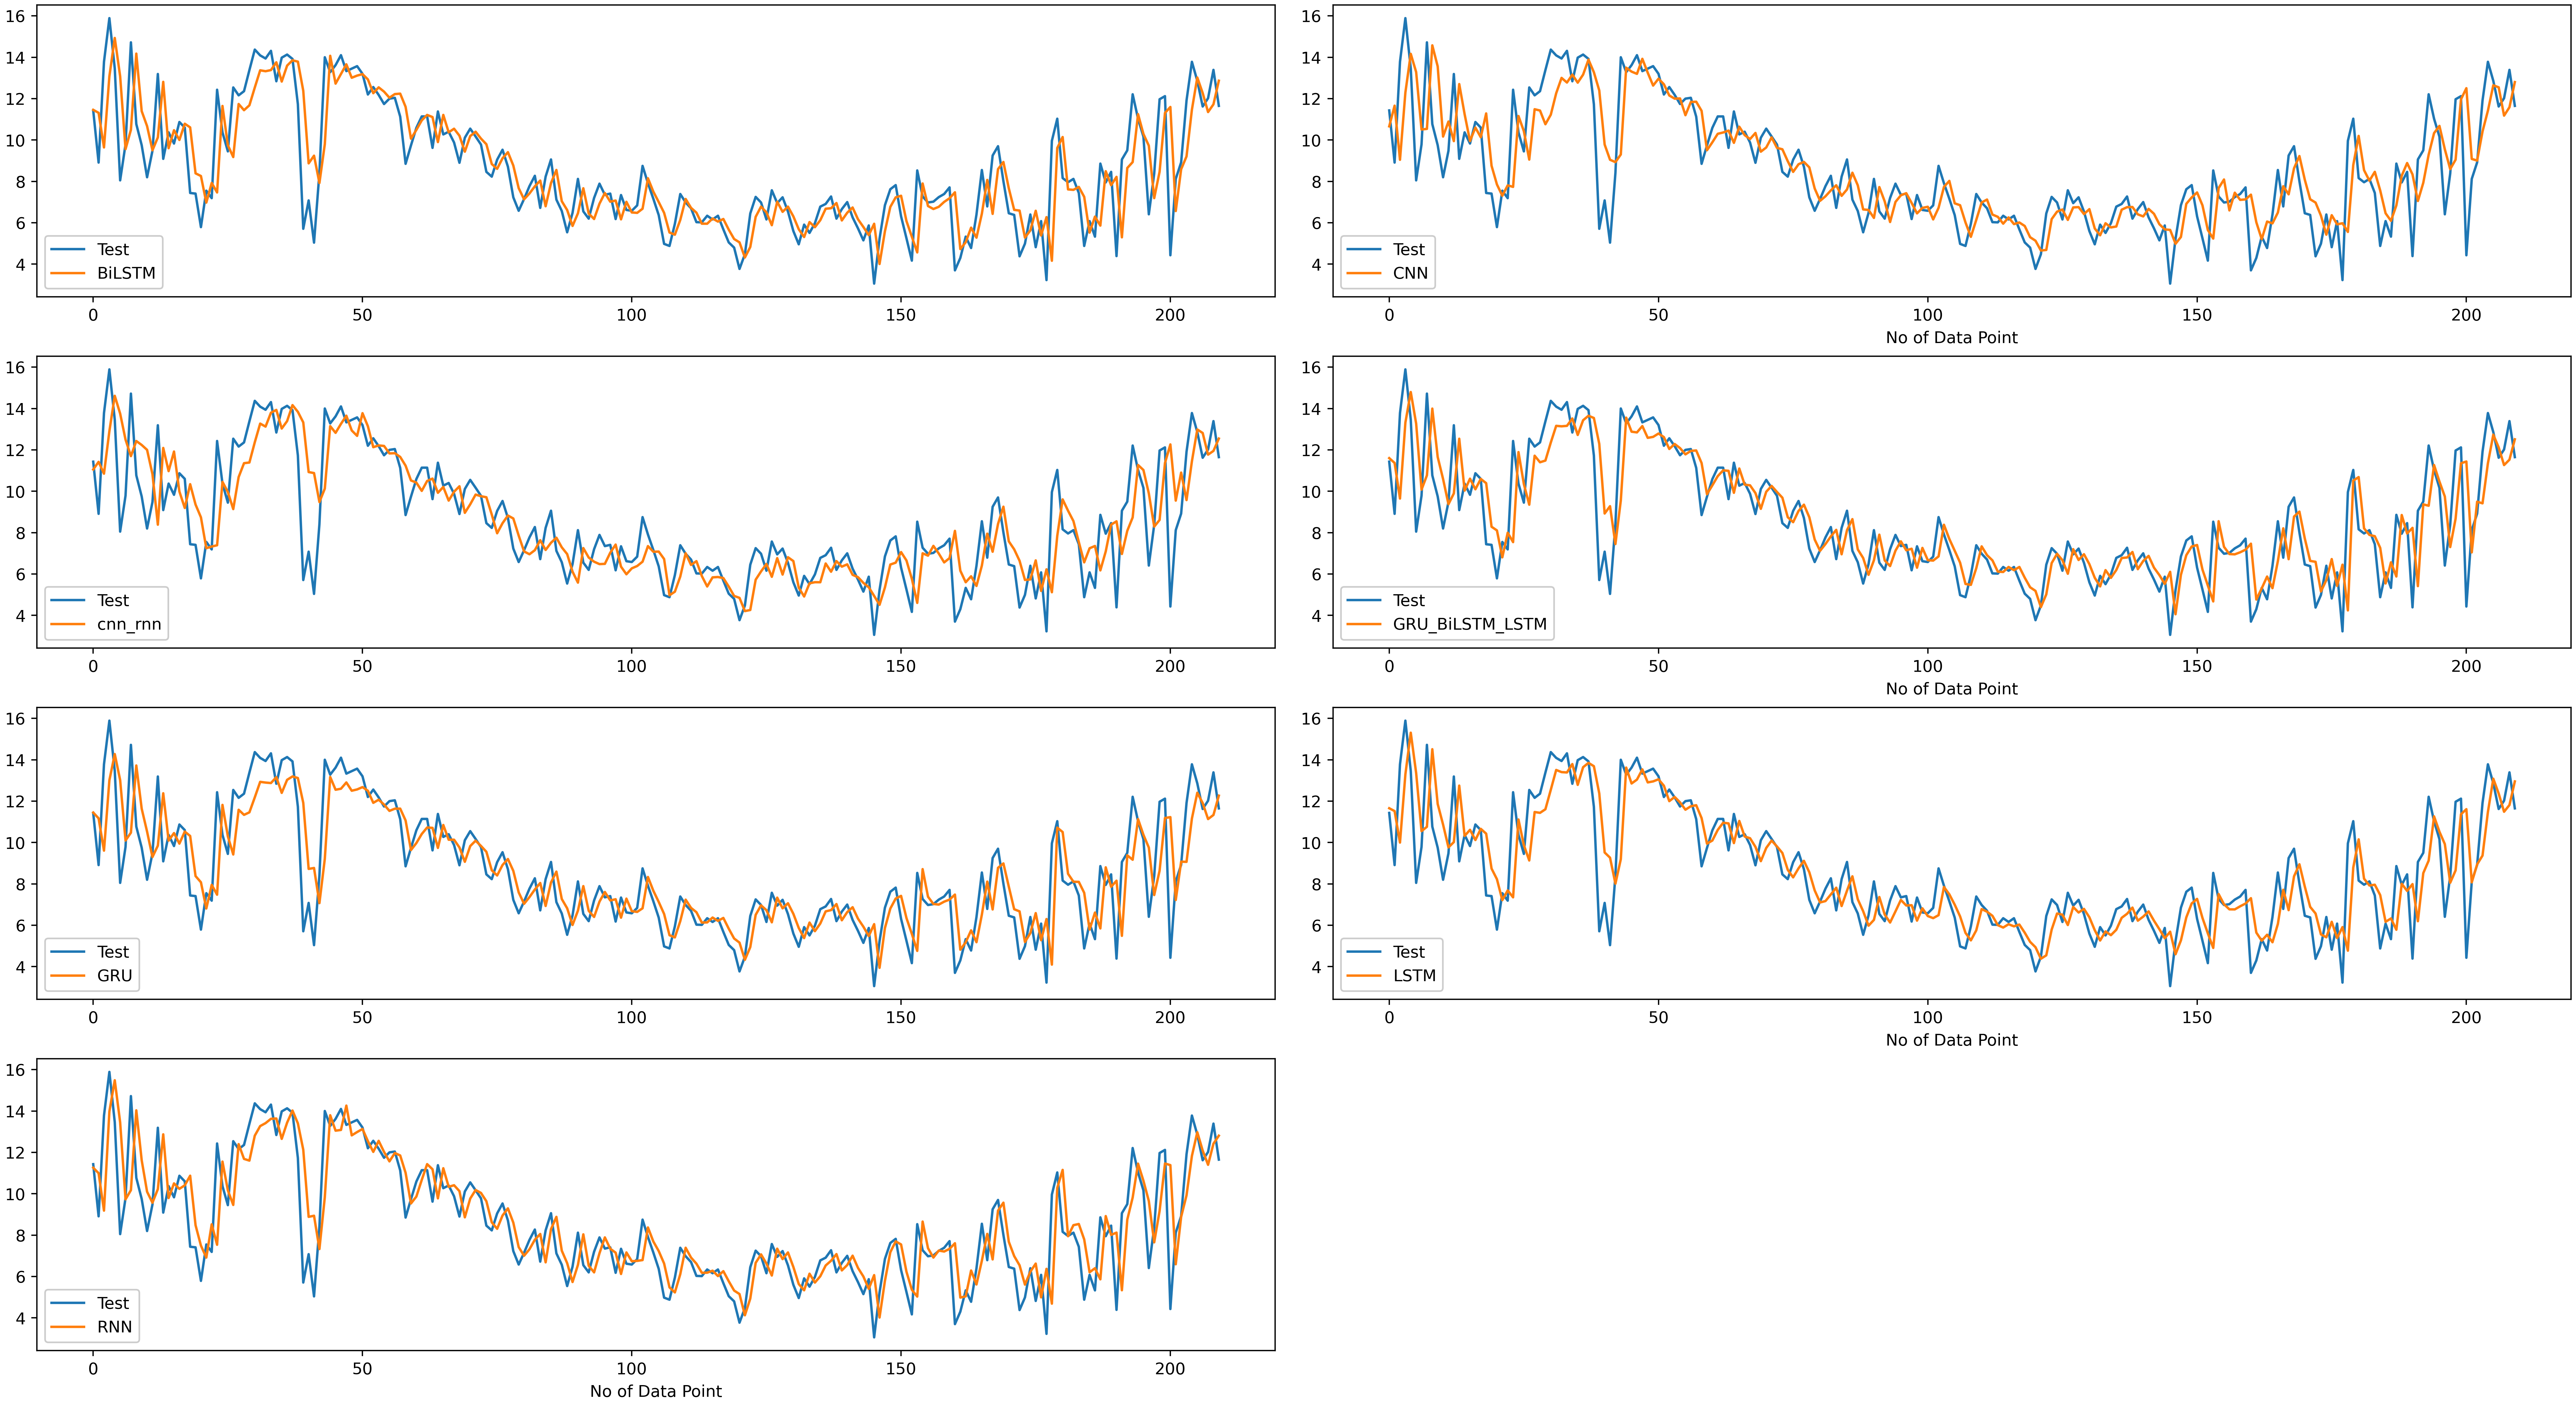
\includegraphics[width=\textwidth]{South Delhi_act vs pred (1)}
      \caption{Line plot Actual vs Prediction}
      \label{Line plot10}
      \end{figure}
      
      \begin{figure}[!ht]
      \centering
      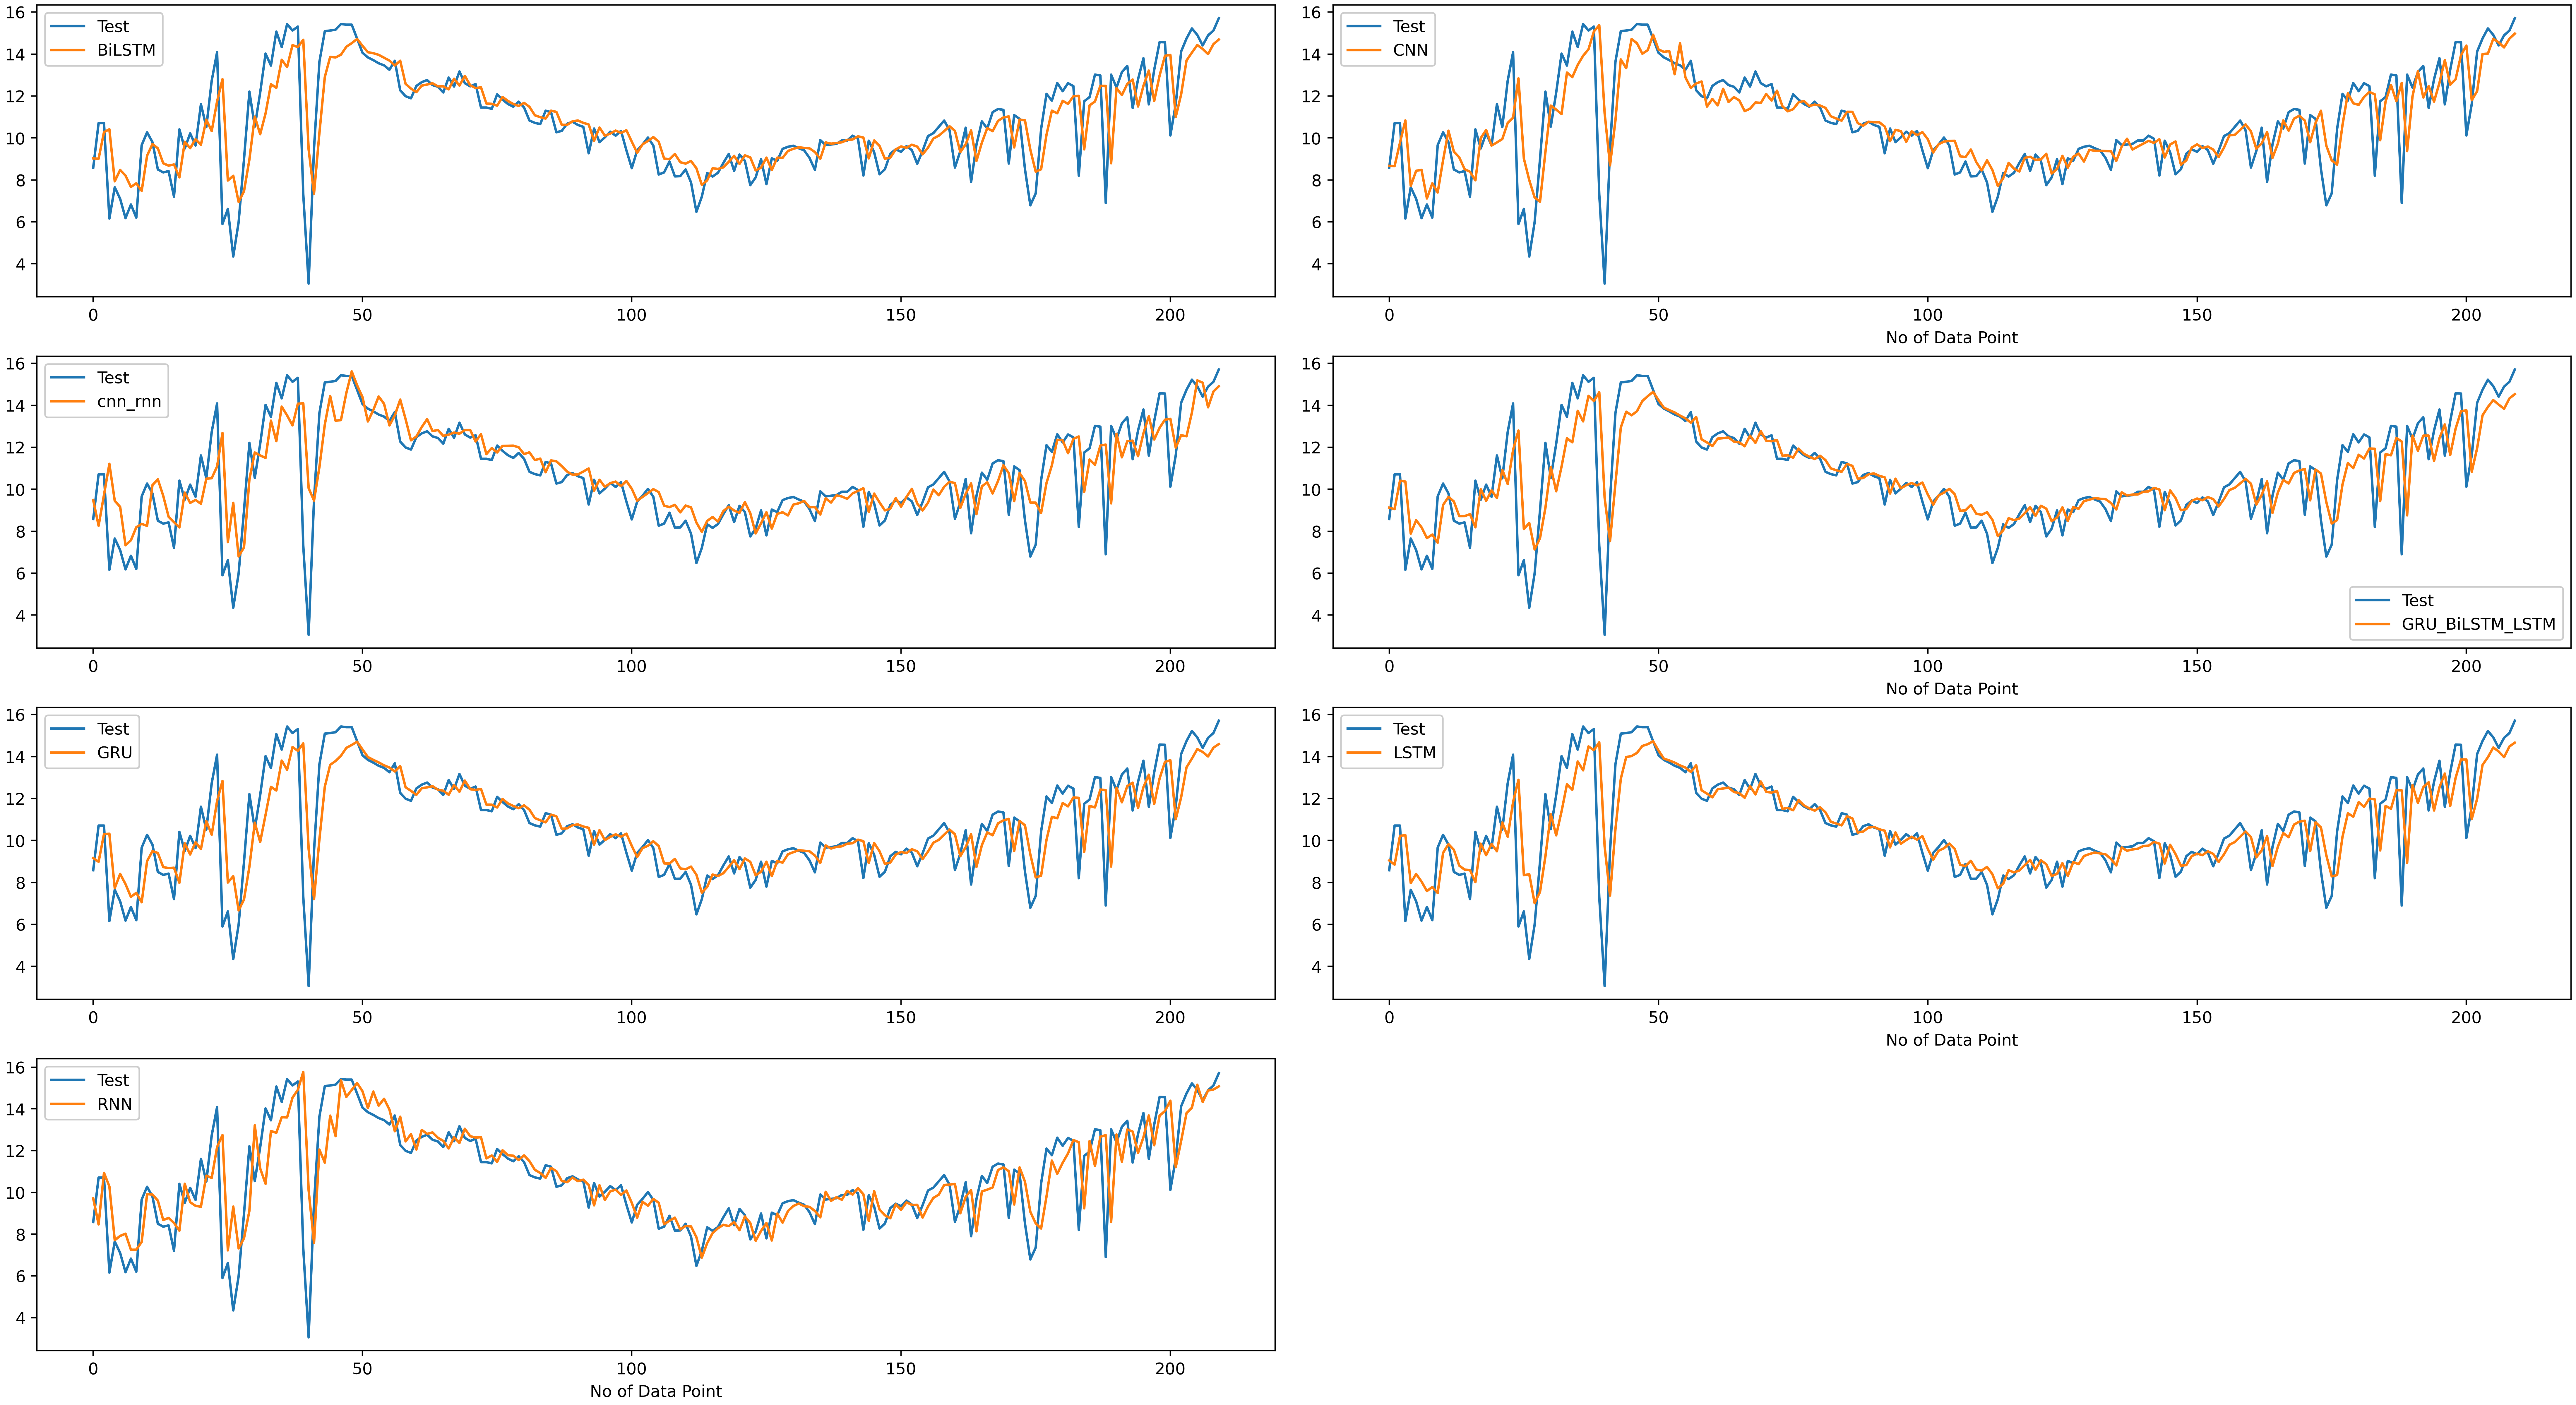
\includegraphics[width=\textwidth]{udaipur_act vs pred}
      \caption{Line plot Actual vs Prediction}
      \label{Line plot11}
      \end{figure}
      
      \begin{figure*}[!ht]
      \centering
      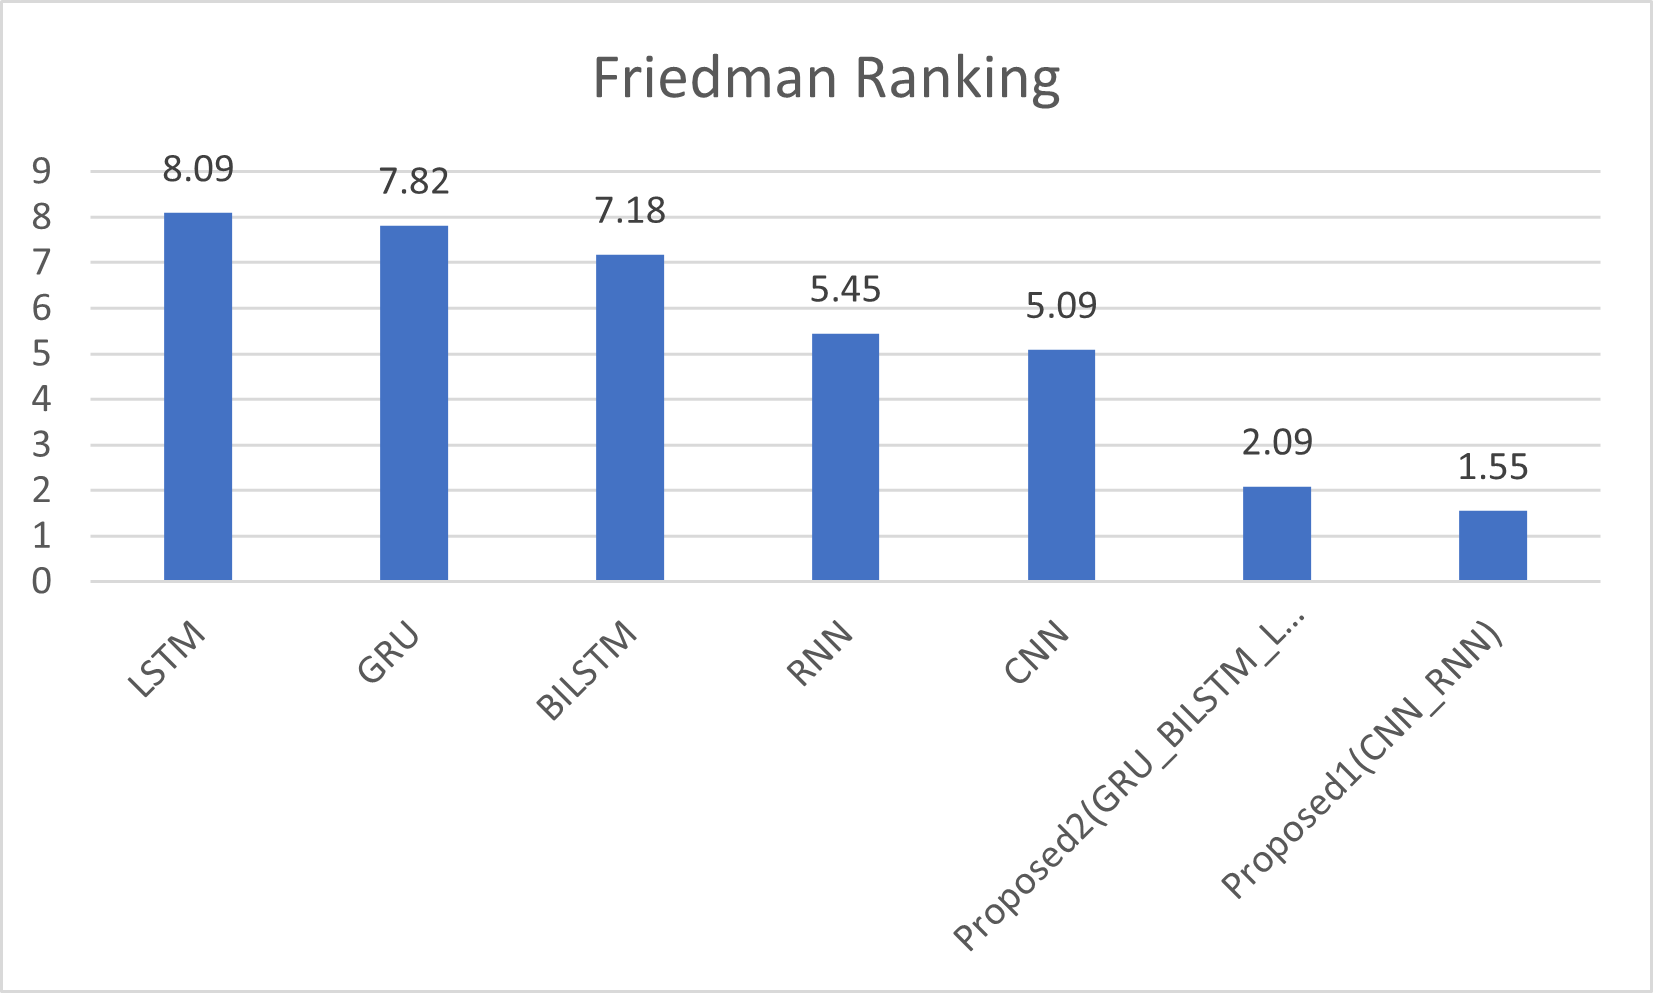
\includegraphics[width=\textwidth]{Friedman test}
      \caption{Plot Friedman Ranking}
      \label{Line plot12}
      \end{figure*}
      



























\section{Conclusions}

\section*{CRediT authorship contribution statement}
\section*{Data availability}
\section*{Acknowledgments}
\label{}

% Numbered list
% Use the style of numbering in square brackets.
% If nothing is used, default style will be taken.
%\begin{enumerate}[a)%\item 
%\item 
%\item 
%\end{enumerate}  

% Unnumbered list
%\begin{itemize}
%\item 
%\item 
%\item 
%\end{itemize}  

% Description list
%\begin{description}
%\item[]
%\item[] 
%\item[] 
%\end{description}  


\begin{comment}

\begin{table}[<options>]
\caption{}\label{tbl1}
\begin{tabular*}{\tblwidth}{@{}LL@{}}
\toprule
  &  \\ % Table header row
\midrule
 & \\
 & \\
 & \\
 & \\
\bottomrule
\end{tabular*}
\end{table}



\end{comment}
% Uncomment and use as the case may be
%\begin{theorem} 
%\end{theorem}

% Uncomment and use as the case may be
%\begin{lemma} 
%\end{lemma}

%% The Appendices part is started with the command \appendix;
%% appendix sections are then done as normal sections
%% \appendix




\label{}

% To print the credit authorship contribution details
\printcredits

%% Loading bibliography style file
%\bibliographystyle{model1-num-names}
\bibliographystyle{cas-model2-names}

% Loading bibliography database
\bibliography{ref}

% Biography
\bio{}
% Here goes the biography details.
\endbio

%\bio{pic1}
% Here goes the biography details.
\endbio

\end{document}

